\documentclass[letterpaper]{article} % DO NOT CHANGE THIS
% AAAI-27 Author Kit (official, https://aaai.org/authorkit27/, AuthorKit27.zip, aaai2027.sty dated 2026-10-21).
% AAAI anonymous workshop manuscript.
\usepackage[submission]{aaai2027}  % DO NOT CHANGE THIS
\usepackage[hyphens]{url}  % DO NOT CHANGE THIS
\usepackage{graphicx} % DO NOT CHANGE THIS
\urlstyle{rm} % DO NOT CHANGE THIS
\def\UrlFont{\rm}  % DO NOT CHANGE THIS
\usepackage{natbib}  % DO NOT CHANGE THIS AND DO NOT ADD ANY OPTIONS TO IT
\usepackage{caption} % DO NOT CHANGE THIS AND DO NOT ADD ANY OPTIONS TO IT
\frenchspacing  % DO NOT CHANGE THIS
\usepackage{algorithm}
\usepackage{algorithmic}
\usepackage{booktabs}
\usepackage{array}
\usepackage{amsmath}
\usepackage{placeins} % \FloatBarrier keeps appendix floats in their sections
\pdfinfo{
/TemplateVersion (2027.1)
}
\setcounter{secnumdepth}{2} % Section numbers enabled (permitted by the template: 0, 1 or 2).

\title{BrickForma: Crystallizing LLM Geometric Knowledge\\into Small Models for Text-to-Brick Assembly}
\author{Anonymous submission}
\affiliations{}

% AAAI sets \@maketitle in the full-width first-page title block.
% Append the teaser inside that block so it precedes the two-column abstract.
\AddToHook{cmd/@maketitle/after}{\par

\begingroup
\centering
% The standalone PDF already supplies a transparency group for its PNG tiles.
\pdfximage width 0.9\textwidth {figure1.pdf}%
\noindent\makebox[\textwidth][c]{\pdfrefximage\pdflastximage}\par
\begin{minipage}{.95\textwidth}
\captionof{figure}{BrickForma overview. (a) Voxel-to-LEGO conversion. (b) Connectivity refinement. (c) Each triplet shows, from left to right, a voxel model from an LLM-authored generator, its converted LEGO assembly, and a BrickForma output (fine-tuned Qwen3-1.7B) for the same category. Brick-type colors are for display only and are not part of the training targets.}
\label{fig:teaser}
\end{minipage}
\par
\endgroup
}

\begin{document}
\maketitle
% Polished sections (proofread by Claude) live in claude/. The original text is preserved in
% main-original.tex, abs-xiao-2.tex, intro-xiao.tex, and the un-suffixed table/figure files.
% Polished version of abs-xiao-2.tex (proofread by Claude). The original file is unchanged.
\begin{abstract}
Geometric spatial reasoning underlies applications ranging from robotics to automated design, yet whether language models can turn a verbal description into a physically connected 3D assembly remains largely unexplored. LEGO\textsuperscript{\tiny\textregistered} brick assembly offers a demanding constructive test of this ability: a short, underspecified prompt leaves dimensions, proportions, and part layout implicit, while a valid assembly must both capture the prompt's semantic intent and satisfy the physical constraints imposed by interlocking studs. We formalize this setting as the \texttt{Text-to-Brick} task and present BrickForma, a framework that crystallizes the geometric knowledge of large language models (LLMs) into a small language model for this task without requiring human-annotated or human-verified 3D shape assets. In BrickForma, executable programs written by LLM agents procedurally generate 80,000 voxel models across 21 categories on a $48\times48\times48$ grid. Each model is paired with five captions of increasing detail, yielding approximately 400,000 geometry-grounded training examples. Connectivity analysis and refinement convert the voxel models into geometrically checked brick targets, of which 79,301 pass all checks, and we fine-tune Qwen3-1.7B to predict brick dimensions and positions from text. Prior systems depend on curated assets: BrickGPT builds on human-annotated ShapeNetCore meshes, and BrickNet relies on human-designed LDraw assemblies. BrickForma instead generates both the voxel geometries and their brick targets programmatically. On 525 shared prompts spanning five description levels, BrickForma's final outputs after refinement and recovery achieve the highest mean VQAScore, PE, and SigLIP2 at each level. The mean invalid-placement ratio is 0.00\% for BrickForma and BrickGPT, and 18.42\% for BrickNet.
\end{abstract}


% Polished version of intro-xiao.tex (proofread by Claude). The original file is unchanged.
\section{Introduction}
Spatial reasoning and geometric understanding are fundamental to human cognition and to artificial intelligence, supporting applications from robotics and navigation to computer-aided design. As large language models (LLMs) have matured, a growing body of work asks whether they can reason about shape, position, and transformation. Recent benchmarks probe this ability through paper folding and unfolding~\cite{zhou2026paperfoldingpuzzle} and through geometry expressed as procedural drawing code~\cite{luo2026geogrambench}, and both report pronounced deficiencies in current models. These studies largely assess spatial reasoning by asking a model to select or compute an answer. A complementary and less examined question is whether a language model can \emph{construct}: given only words, can it produce a three-dimensional object whose parts are correctly sized, correctly placed, and physically joined?

LEGO brick assembly makes this question concrete. A concise request such as \emph{a simple chair} identifies an object category but leaves its dimensions, proportions, and part layout largely unspecified. Answering it requires three coupled forms of geometric spatial reasoning. The model must complete the missing geometry from prior knowledge of what the object looks like. It must discretize that geometry into pieces of fixed dimensions at integer positions on a grid. And it must respect the difference between spatial adjacency and stud connectivity: pieces that touch side by side do not hold together unless they interlock vertically through studs. We call this setting the \texttt{Text-to-Brick} task: translating a natural-language description, at any level of detail, into a set of LEGO brick placements that reproduces the described shape as a single connected assembly. Because every output can be checked for coverage, bounds, and connectivity, the task offers a verifiable test of whether linguistic knowledge has become spatial structure.

Prior work has shown that language models can be trained for this task. BrickGPT~\cite{brickgpt} learns autoregressive brick-placement sequences and applies validity checks with physics-aware rollback during inference. BrickNet~\cite{bricknet} adopts a graph-based representation that supports a broader range of parts and connection types. Two questions remain open. \textbf{(Q1)} How well do generators translate \emph{limited} linguistic information into object geometry? Pooled scores hide this: only a level-wise evaluation (Table~\ref{tab:level-results}) shows, for example, that BrickNet trails BrickForma on mean VQAScore, PE, and SigLIP2 even at the two shortest description levels, L1 and L2. \textbf{(Q2)} Can LLM-assisted programs encode the geometric details omitted from concise prompts in a form suitable for training a compact model?

We present BrickForma, which uses executable programs to generate training examples for a compact text-to-brick model. With the assistance of GPT-6.1 Sol, we develop parametric programs that vary object proportions, part dimensions, openings, and support arrangements to synthesize voxel shapes in batches. Each program specifies the structure of an object family and exposes its geometric degrees of freedom as parameters. The source collection contains 80,000 models across 21 categories on a $48^3$ grid. Each model is paired with five levels of description that progressively add structural, geometric, proportional, and appearance information. The resulting approximately 400,000 caption records link concise requests and detailed specifications to shared geometry, providing supervision for prompts with different amounts of geometric detail.

Turning voxel shapes into brick targets is where spatial adjacency and stud connectivity must be separated: pieces can cover a connected voxel volume and touch side by side without forming any stud connection. Our conversion pipeline combines same-color brick placement, connection analysis, and local refinement to construct geometrically checked target layouts, and it records every change to the source voxels in the derived models. The integrated dataset release contains 79,301 models that pass its dataset-level geometric checks. We fine-tune Qwen3-1.7B~\cite{qwen3} with low-rank adaptation~\cite{lora} on caption--placement pairs to predict brick dimensions and positions.

Geometric refinement complements the small model's predictions with explicit structural enforcement. From the supported, in-bounds portions of the predicted placements, the pipeline forms a voxel union and uses mixed-integer linear programming to find an exact-cover layout that forms a single stud-connected component. Independent coverage and connectivity checks then verify the refined layout. This design gives each half of the task to the component suited to it: the language model decides what shape a description denotes, and the solver decides how that shape holds together.

We evaluate BrickForma against BrickGPT and BrickNet on 525 shared prompts spanning five description levels. BrickForma's final outputs after refinement and recovery achieve the highest mean VQAScore, PE, and SigLIP2 at every level, including the shortest descriptions. The mean invalid-placement ratio is 0.00\% for BrickForma and BrickGPT, and 18.42\% for BrickNet. Reporting all five levels links the multi-level data design to an explicit assessment of how generation changes with the amount of descriptive detail.

In summary, our main contributions are as follows:

\textbf{LLM-assisted training data for a compact model.}
We use executable parametric programs to generate voxel shapes and their descriptions, convert the shapes into geometrically checked brick layouts, and fine-tune a 1.7B-parameter model on the resulting caption--placement pairs. On the 525 shared prompts, BrickForma's final outputs reach a mean VQAScore of 0.0872, compared with 0.0666 for BrickGPT, an absolute difference of 0.0206 (30.9\% relative).

\textbf{A multi-level dataset for evaluating alignment across levels of descriptive detail.}
Our pipeline generates 80,000 source voxel models with five description levels each; in the integrated release, 79,301 of them yield brick layouts that pass the geometric checks. Level-wise evaluation against BrickGPT and BrickNet, covering text--image alignment and invalid placements from concise prompts to detailed specifications, shows that BrickForma achieves the highest mean alignment scores at all five levels.


\begin{figure*}[t]
\centering
\begingroup
% Use the existing PDF transparency group for the model renders.
\pdfximage width \textwidth {figure2.pdf}%
\pdfrefximage\pdflastximage\endgroup
\caption{Data-construction workflow. GPT-6.1 Sol assists in writing parametric programs that produce voxel shapes and their captions. After deduplication, the shapes are converted to bricks, refined, and checked before export. Dashed arrows trace contact screening and its recorded status. Brick colors follow the legend in Figure~\ref{fig:teaser}.}
\label{fig:data-workflow}
\end{figure*}

% Polished Related Work section (proofread by Claude). Original text is in main-original.tex.
\section{Related Work}
\paragraph{Brick assembly and generation.}
Prior work formulates brick assembly as graph generation, sequential construction, or structural understanding~\cite{thompson2020lego,brickbybrick,breakandmake}. BrickGPT~\cite{brickgpt} predicts autoregressive placement sequences and validates candidate bricks during decoding, while BrickNet~\cite{bricknet} adopts an assembly-graph representation over a broader catalog of parts and connectors. Rather than relying solely on autoregressive decoding or graph prediction to maintain structural validity, BrickForma predicts absolute grid placements for rectangular footprints and delegates global stud connectivity to exact-cover voxel reconstruction.

\paragraph{Stability analysis.}
StableLEGO introduces a force-balance model for evaluating block-stacking assemblies~\cite{stablelego}. In BrickForma, inference-time refinement enforces stud connectivity and exact voxel coverage, while dataset-level contact screening applies complementary force and ground-contact assumptions to flag physically plausible structures (Appendix~\ref{app:dataset}).


% Polished Dataset Construction section (proofread by Claude). Original text is in main-original.tex.
\section{Dataset Construction}
\label{sec:dataset}
\subsection{Parametric Voxel Generation}
To crystallize broad geometric priors into explicit supervision, GPT-6.1 Sol assists in authoring analytic parametric generator programs for 21 object categories, each partitioned into 40 structural families (47--48 instances per family in each 40,000-model shard). For every instance, a planning module samples independent design parameters, which govern category-specific components, proportions, openings, and support structures. It then deterministically rasterizes the geometry onto a $48^3$ grid ($Y{=}0$ is ground contact) and derives the L1--L5 captions from the same underlying plan. Instead of applying random cell deletion, cavity filling, or post-hoc bridges, density adjustments regenerate the entire shape from its continuous parameters until automated checks confirm 750--1,250 occupied voxels forming a single six-neighbor connected component. Exact and canonical occupancy hashes over the 48 axis-permutation and sign transforms confirm zero cross-shard duplicates, and the geometry plan and version identifiers are stored with each record (Figure~\ref{fig:data-workflow}, where \texttt{shape(params)} denotes the analytic shape and \texttt{emit(x,y,z)} records occupied voxel coordinates).

BrickForma pairs each shape with five bilingual descriptions. L1 names the object and its primary parts, and L2--L5 progressively add structural, proportional, appearance, and viewpoint details about the same source geometry (Appendix~\ref{app:dataset} gives a birdhouse example).

\subsection{Voxel-to-Brick Conversion and Checks}
Converting a connected voxel volume into a buildable brick target requires separating mere spatial adjacency from vertical stud connectivity. Our pipeline tiles each layer with same-color rectangular bricks and analyzes the resulting stud-connected components. When ungrounded fragments arise, local refinement modifies the layout and logs every voxel edit against the source shape, raising the geometry-pass count from 65,503 to 79,298 (13,795 recovered failures). Across the corpus, refinement adds 228,582 voxels and removes 125, and 31,532 passing models require no edits at all.

For challenging layouts, conversion falls back to layer-wise exact-cover search or to a mixed-integer linear program (MILP) that explicitly enforces a stud path to the ground. A minimum-remaining-values (MRV) heuristic branches on the uncovered voxel with the fewest valid candidate bricks. When greedy placement failed the geometric audit, the initial release also used bounded beam search, ranking partial layouts by uncovered voxels and remaining stud components.

Release-level verification confirms that the target voxels form a single six-neighbor component, that every brick component is grounded, and that the brick assembly exactly covers the derived target. Release-level checks allow several independently grounded components; inference-time refinement enforces a single component. Separately, a self-weight screen evaluates the final assembly and, where feasible, each bottom-up prefix of completed layers. It records the tipping margin and estimates the per-stud tensile demand when compression alone cannot balance gravity (Appendix~\ref{app:dataset}).

\subsection{Integrated Release and Training Corpus}
The full refined release passes 79,298 models and leaves 702 geometry failures. A revised release of the batch-B piano models passes all 1,905 piano slots, compared with 1,902 in the full refined release, so the integrated release contains $79{,}298-1{,}902+1{,}905=79{,}301$ passing models. Table~\ref{tab:training-data} summarizes the release counts and the fine-tuning corpus.
\begin{table}[t]
\centering
\small
\setlength{\tabcolsep}{4pt}
\begin{tabular}{lr}
\toprule
\multicolumn{2}{l}{\emph{Dataset (release reports)}} \\
\midrule
Source models / categories / grid & 80,000 / 21 / $48^3$ \\
%Bilingual 
Caption records & 400,000 \\
Failing in full refined release & 702 (0.88\%) \\
Passing in full refined release & 79,298 \\
Piano models restored by revised release & 3 \\
Integrated passing models & 79,301 \\
\midrule
\multicolumn{2}{l}{\emph{Fine-tuning corpus}} \\
\midrule
%396,610 ?
Voxel-model \& caption samples & 396,610 \\ % Training manifest confirmation pending
Training / %validation 
test samples & 356,955 / 39,655 \\
%xiao
% Tokens over 3 epochs & 2,228,044,818 \\ % Training manifest confirmation pending
\bottomrule
\end{tabular}
\caption{Dataset and fine-tuning corpus. The two blocks are counted separately: the upper block comes from the dataset release reports, and the lower block is as recorded for the fine-tuning run.}
\label{tab:training-data}
\end{table}



% Polished BrickForma Text-to-Brick Model section (proofread by Claude). Original text is in main-original.tex.
\section{BrickForma Text-to-Brick Model}
\label{sec:model}
\subsection{Fine-Tuning}
\label{sec:training}
We fine-tune Qwen3-1.7B with LoRA on English L1--L5 captions paired with their checked brick layouts. We split the data 9:1 at the model level, so all five descriptions of a shape fall in the same partition. The $48^3$ workspace uses 20 oriented footprints (the 11 brick sizes in their distinct planar rotations). Each instruction lists the allowed brick dimensions, and the target gives one placement per line, such as $2{\times}4\ (x,y,z)$, ordered first by Y and then by X. Targets encode pure geometry, with no color tokens.

Training follows the BrickGPT Qwen3 recipe~\cite{brickgpt} (Table~\ref{tab:finetune-config}), with unpacked sequences to preserve caption boundaries. The run completed 133,860 steps in 25.3 hours on eight GPUs. Validation loss reached its minimum of 0.0308 at step 79,000, which we release as the checkpoint, and rose slightly to 0.0339 by the end of epoch 3 (Appendix~\ref{app:training}).
\begin{table}[t]
\centering
\small
\setlength{\tabcolsep}{3pt}
\begin{tabular}{@{}l>{\raggedright\arraybackslash}p{0.58\linewidth}@{}}
\toprule
Item & Value \\
\midrule
Base model & Qwen3-1.7B (bf16) \\
Adaptation & LoRA, $r=16$, $\alpha=32$, dropout $0.05$, all linear layers \\
Optimization & LR $10^{-4}$, cosine, 100 warm-up steps, 3 epochs \\
Batch / max length & effective 8 (8 GPUs $\times$ 1) / 8,192 \\
Hardware & DDP, 8$\times$RTX 4090D (24\,GB) \\
Released checkpoint & step 79,000 (best validation loss) \\
Software & transformers 4.51.3, trl 0.17.0, peft 0.15.2 \\
\bottomrule
\end{tabular}
\caption{Fine-tuning configuration (details in Appendix~\ref{app:training}).}
\label{tab:finetune-config}
\end{table}


\subsection{Inference and Refinement}
As outlined in Algorithm~\ref{alg:inference-refinement}, decoding runs with thinking disabled, temperature $0.7$, top-$p$ $0.9$, and an 8,192-token budget, trying seeds 42, 104, and 2026 in order. A draft is complete once it emits an end-of-sequence token. The pipeline stops at the first completed draft that passes the geometry validator; if none passes, it takes the completed draft with the fewest validator errors, and if no draft completes, it reports a failure. Here $\mathrm{Err}(B)$ counts the validator errors in a layout $B$ (unsupported footprints, out-of-bounds placements, and overlaps), so a draft is valid when $\mathrm{Err}(B)=0$, and $\kappa(B)$ is the number of stud-connected components. A valid draft with $\kappa(B)=1$ is returned unchanged.

For all other drafts, we isolate the semantic shape proposal by forming the in-bounds voxel union $C$ of all placements with a supported footprint (counting overlaps once) and hand structural assembly to an MILP solver. The solver seeks an exact cover of $C$ that forms a single stud-connected component, under time limits of 12, 60, and 180 seconds, and an independent audit then checks placement validity, coverage, and connectivity. Because the cover is exact, a refined layout occupies exactly the voxel set $C$ derived from its draft. If all time limits are exhausted, the pipeline keeps the raw draft and queues a reseed; optional recovery runs extend the budget to 600 seconds or sample additional seeds. Throughout the evaluation, we call pre-solver model outputs \emph{raw} and solver-reconstructed outputs \emph{refined} (Appendix~\ref{app:eval} gives the exact-cover constraints).
% Algorithm 1, version 2 (revised by Claude). Version 1 is kept in algorithm1-v1-claude.tex.
% Changes from v1:
%  - Only completed drafts enter the candidate set; the empty-set sentinel B = \emptyset is gone,
%    so an empty layout can no longer be confused with "no draft selected".
%  - Err(.) and kappa(.) take a layout (v1 applied Err to a (layout, report) pair);
%    "valid" is defined as Err = 0, so rep.valid is no longer a separate notion.
%  - The selection rule (first valid draft, else fewest errors) is one arg-min, equivalent to v1.
%  - Statuses distinguish RAW (returned unchanged) from REFINED (solver output),
%    matching the raw/refined terms used in the evaluation.
%  - The voxel union C is written out (in-bounds voxels of placements with a supported footprint).
%  - Err, kappa, and Audit are defined in the Section 4.2 text (model-claude.tex).
%  - Recovery runs (extra seeds, 600 s budget) appear as a comment, as in Section 4.2.
% TO CONFIRM AGAINST CODE: tie-breaking among equal-error drafts; behaviour when C is empty;
% whether a FAILED prompt also queues a reseed.
\begin{algorithm}[tb]
\caption{BrickForma inference and refinement}
\label{alg:inference-refinement}
\small\raggedright
\begin{algorithmic}[1]
\REQUIRE prompt $c$; fine-tuned model $\theta$; footprint library $\mathcal{L}$ ($|\mathcal{L}|{=}20$); grid $G{=}\{0,\dots,47\}^3$; seeds $S{=}(42,104,2026)$; MILP time limits $T{=}(12,60,180)$\,s
\ENSURE $(B_{\mathrm{out}},\textit{status})$, $\textit{status}\in\{\textsc{Raw},\textsc{Refined},\textsc{Draft},\textsc{Failed}\}$
\STATE $\mathcal{A} \gets \emptyset$ \COMMENT{completed drafts}
\FOR{$s \in S$ (in order)}
  \STATE $(B_s,\textit{done}) \gets \mathrm{Parse}(\mathrm{Decode}_{\theta}(c;\, s))$
  \IF{$\textit{done}$}
    \STATE $\mathcal{A} \gets \mathcal{A} \cup \{B_s\}$
    \IF{$\mathrm{Err}(B_s)=0$}
      \STATE \textbf{break} \COMMENT{first valid draft}
    \ENDIF
  \ENDIF
\ENDFOR
\IF{$\mathcal{A}=\emptyset$}
  \RETURN $(\emptyset,\ \textsc{Failed})$ \COMMENT{no draft completed}
\ENDIF
\STATE $B \gets \arg\min_{B' \in \mathcal{A}} \mathrm{Err}(B')$
\IF{$\mathrm{Err}(B)=0 \land \kappa(B)=1$}
  \RETURN $(B,\ \textsc{Raw})$ \COMMENT{valid and connected}
\ENDIF
\STATE $C \gets \bigcup_{b \in B,\ \mathrm{fp}(b)\in\mathcal{L}} \bigl(\mathrm{vox}(b) \cap G\bigr)$ \COMMENT{overlaps count once}
\FOR{$\tau \in T$}
  \STATE $B^{*} \gets \mathrm{SolveMILP}(C,\mathcal{L};\ \tau)$ \COMMENT{exact cover, $\kappa{=}1$ (App.~\ref{app:eval})}
  \IF{$B^{*}$ found $\land\ \mathrm{Audit}(B^{*},C)$}
    \RETURN $(B^{*},\ \textsc{Refined})$
  \ENDIF
\ENDFOR
\STATE $\mathrm{QueueReseed}(c)$ \COMMENT{recovery: new seeds or 600\,s}
\RETURN $(B,\ \textsc{Draft})$ \COMMENT{keep the raw draft}
\end{algorithmic}
\end{algorithm}



% Polished Comparative Evaluation section (proofread by Claude). Original text is in main-original.tex.
\section{Comparative Evaluation}
\label{sec:eval}
\subsection{Setup and Metrics}
\label{sec:setup}
We evaluate BrickForma against BrickGPT and BrickNet on 525 shared prompts spanning 21 categories and five description levels (105 prompts per level). The main comparison uses one output per system and prompt, for 1,575 LDraw exports. For BrickForma we score the final layouts after refinement and recovery. They include refined originals, retained originals, and regenerated layouts. BrickGPT and BrickNet use the delivered outputs from the original comparison. Appendix~\ref{app:eval} details the provenance and the separate structural diagnostic.

\emph{Text--image alignment.}
Each export is rendered in a uniform yellow material from eight $512{\times}512$ orthographic views, spaced $45^\circ$ apart in azimuth at $25^\circ$ elevation. Each alignment score takes the maximum over views and is then averaged across prompts. VQAScore~\cite{vqascore} is the first-token probability of \textquotedblleft Yes\textquotedblright\ under Qwen2.5-VL-7B-Instruct~\cite{qwen25vl}; PE~\cite{pe} is the cosine similarity between normalized image and text embeddings; and SigLIP2~\cite{siglip2} is the sigmoid of the image--text logit.

\emph{Invalid placements.}
For an export with $n$ placements in file order, let $I_i$ indicate whether placement $i$ violates BrickNet's inset collision kernel~\cite{bricknet} given the preceding placements. We report the mean per-export invalid-placement ratio $P_{\mathrm{inv}}=n^{-1}\sum_{i=1}^{n}I_i$.

\subsection{Main Results}
\begin{table}[t]
\centering\small
\setlength{\tabcolsep}{3pt}
\begin{tabular}{lrrrr}
\toprule
System & $P_{\mathrm{inv}}\downarrow$ & VQAScore $\uparrow$ & PE $\uparrow$ & SigLIP2 $\uparrow$ \\
\midrule
BrickForma & \textbf{0.00\%} & \textbf{0.0872} & \textbf{0.1581} & \textbf{0.0452} \\
BrickGPT & \textbf{0.00\%} & 0.0666 & 0.1440 & 0.0194 \\
BrickNet & 18.42\% & 0.0201 & 0.1187 & 0.0011 \\
\bottomrule
\end{tabular}
\caption{Mean scores on 525 shared prompts. BrickForma uses final outputs after refinement and recovery. Bold marks the best mean, including ties.}
\label{tab:main}
\end{table}

Across all 525 prompts, BrickForma's final outputs achieve the highest mean VQAScore (0.0872), PE (0.1581), and SigLIP2 (0.0452) (Table~\ref{tab:main}), outperforming BrickGPT on 372, 341, and 323 prompts, respectively. All six paired alignment comparisons are statistically significant after Holm correction (Appendix~\ref{app:eval}). BrickForma and BrickGPT both score 0.00\% mean $P_{\mathrm{inv}}$, while BrickNet scores 18.42\%. The zero-invalid-placement counts are 525 for BrickForma, 525 for BrickGPT, and 139 for BrickNet (Figure~\ref{fig:comparison-zero-invalid}). Figures~\ref{fig:comparison-means} and~\ref{fig:comparison-distributions} show pooled means and score distributions.

\paragraph{Comparison with the untuned backbone.}
To measure the effect of parametric supervision, and thus to address \textbf{(Q2)}, we compare against untuned Qwen3-1.7B on 260 matched prompts, assigning zero alignment scores whenever it fails to produce a scorable layout. Mean VQAScore, PE, and SigLIP2 rise from 0.0008, 0.0354, and 0.0014 for the untuned backbone to 0.0649, 0.1564, and 0.0328 for raw BrickForma before geometric refinement (Appendix~\ref{app:eval}).

\subsection{Performance across Description Levels}
\begin{table*}[t]
\centering\small
\setlength{\tabcolsep}{3pt}
\begin{tabular}{lrrlrrrr}
\toprule
Level & $n$ & Words & System & $P_{\mathrm{inv}}\downarrow$ & VQAScore $\uparrow$ & PE $\uparrow$ & SigLIP2 $\uparrow$ \\
\midrule
L1 & 105 & 13.6 & BrickForma & \textbf{0.00\%} & \textbf{0.1593} & \textbf{0.1386} & \textbf{0.0171} \\
 &  &  & BrickGPT & \textbf{0.00\%} & 0.1296 & 0.1302 & 0.0087 \\
 &  &  & BrickNet & 18.59\% & 0.0346 & 0.1051 & 0.0005 \\
\midrule
L2 & 105 & 26.4 & BrickForma & \textbf{0.00\%} & \textbf{0.1308} & \textbf{0.1474} & \textbf{0.0329} \\
 &  &  & BrickGPT & \textbf{0.00\%} & 0.0938 & 0.1338 & 0.0206 \\
 &  &  & BrickNet & 18.35\% & 0.0394 & 0.1030 & 0.0008 \\
\midrule
L3 & 105 & 37.5 & BrickForma & \textbf{0.00\%} & \textbf{0.1126} & \textbf{0.1503} & \textbf{0.0452} \\
 &  &  & BrickGPT & \textbf{0.00\%} & 0.0863 & 0.1415 & 0.0178 \\
 &  &  & BrickNet & 22.98\% & 0.0209 & 0.1113 & 0.0012 \\
\midrule
L4 & 105 & 52.5 & BrickForma & \textbf{0.00\%} & \textbf{0.0189} & \textbf{0.1803} & \textbf{0.0753} \\
 &  &  & BrickGPT & \textbf{0.00\%} & 0.0148 & 0.1605 & 0.0338 \\
 &  &  & BrickNet & 17.24\% & 0.0025 & 0.1376 & 0.0011 \\
\midrule
L5 & 105 & 78.8 & BrickForma & \textbf{0.00\%} & \textbf{0.0144} & \textbf{0.1738} & \textbf{0.0554} \\
 &  &  & BrickGPT & \textbf{0.00\%} & 0.0086 & 0.1542 & 0.0162 \\
 &  &  & BrickNet & 14.95\% & 0.0030 & 0.1363 & 0.0020 \\
\bottomrule
\end{tabular}
\caption{Mean scores by description level. Each level has 105 prompts per system. Words is the mean English word count. BrickForma uses final outputs after refinement and recovery. Bold marks the best mean.}
\label{tab:level-results}
\end{table*}

Addressing \textbf{(Q1)}, the final BrickForma outputs lead on all three mean alignment metrics at each description level (Table~\ref{tab:level-results} and Figure~\ref{fig:comparison-levels}). At L1, mean VQAScore is 0.1593 for BrickForma, 0.1296 for BrickGPT, and 0.0346 for BrickNet. BrickForma and BrickGPT both score 0.00\% mean $P_{\mathrm{inv}}$ at every level. Figure~\ref{fig:gallery} shows qualitative L1 and L2 examples under matched rendering conditions.

\begin{figure*}[t]
\centering
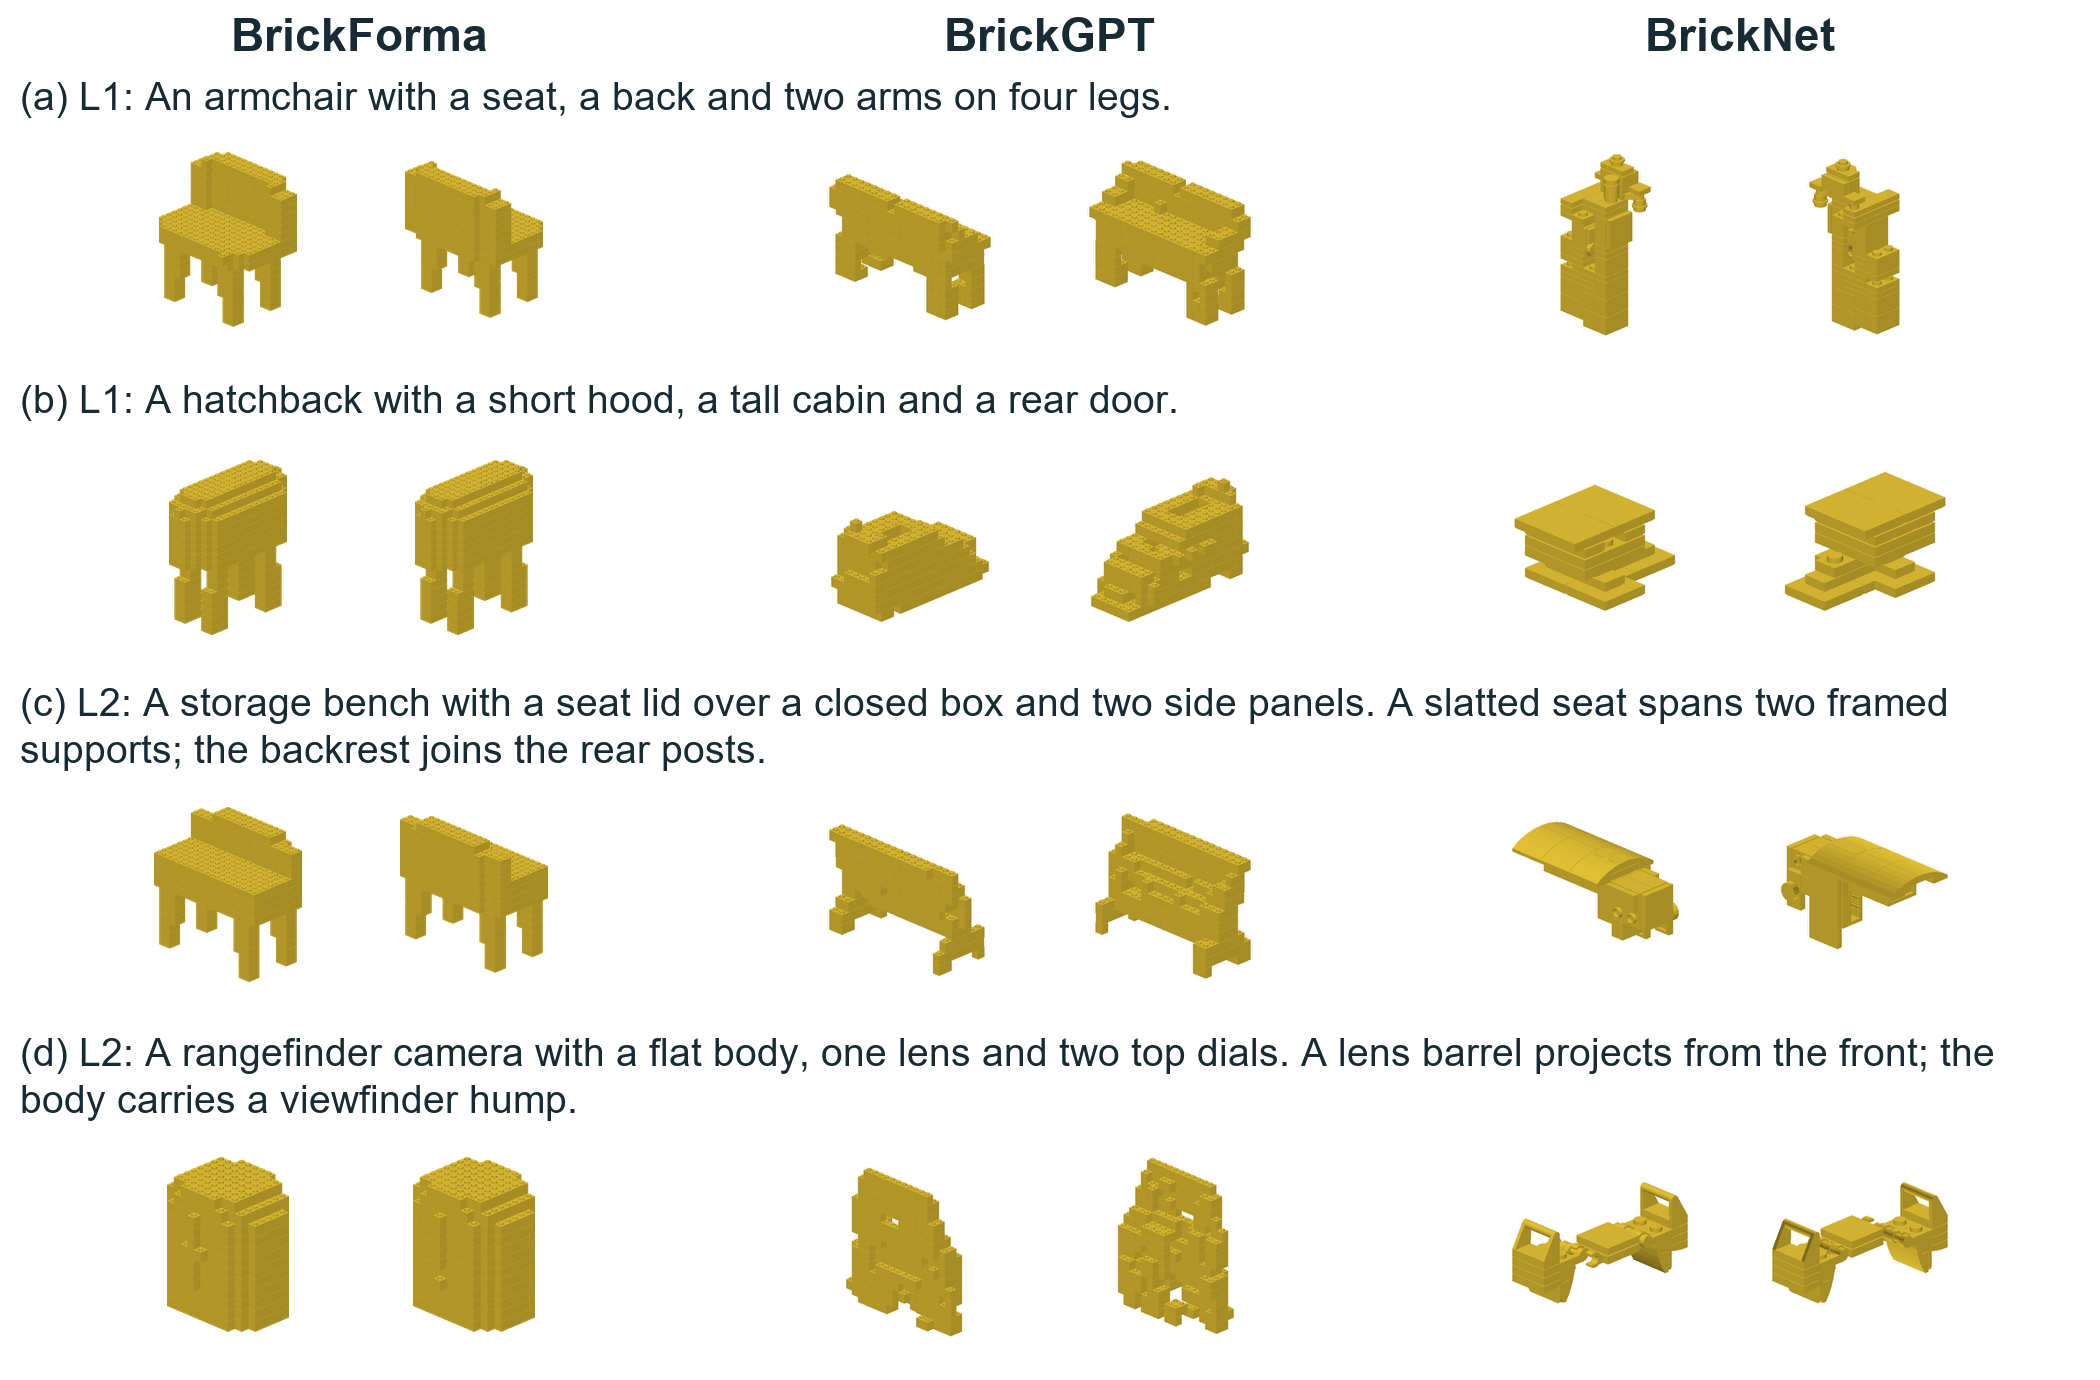
\includegraphics[width=\textwidth]{figures/matched_short_prompts_20261119.png}
\caption{Four examples from the matched evaluation, with the same prompts, render settings, and azimuths ($45^\circ$ and $225^\circ$) for all systems. BrickForma shows the final outputs after refinement and recovery. The highest VQAScore goes to BrickForma for the armchair and the storage bench, to BrickGPT for the hatchback, and to BrickNet for the camera.}
\label{fig:gallery}
\end{figure*}


\subsection{Raw versus Final Outputs}
On the 525 main-benchmark prompts, BrickForma's mean $P_{\mathrm{inv}}$ falls from 0.79\% in the delivered raw outputs to 0.00\% in the final outputs. The number of layouts without invalid placements rises from 331 to 525. The mean VQAScore, PE, and SigLIP2 increase by 0.0006, 0.0013, and 0.0004, respectively. This same-prompt comparison measures the full final-output pipeline, including regeneration on 46 prompts.

\begin{table}[t]
\centering
\small
\begin{tabular}{lrr}
\toprule
Metric & Raw & Refined \\
\midrule
$P_{\mathrm{inv}}$ $\downarrow$ & 0.1897\% & 0.0000\% \\
VQAScore $\uparrow$ & 0.2065 & 0.2071 \\
PE $\uparrow$ & 0.1858 & 0.1859 \\
SigLIP2 $\uparrow$ & 0.1379 & 0.1261 \\
Mean parts & 178.7 & 421.2 \\
\bottomrule
\end{tabular}
\caption{Raw versus refined BrickForma outputs on 110 pairs from the earlier comparison. Each pair shares the same prompt, model identifier, and caption.}
\label{tab:raw-refined}
\end{table}

An earlier 114-prompt comparison provides 110 raw/refined pairs that share a prompt and model identifier (Table~\ref{tab:raw-refined}). Refinement eliminates invalid placements ($P_{\mathrm{inv}}$ drops from 0.1897\% to 0.0000\%) and raises the mean part count from 178.7 to 421.2. VQAScore and PE remain essentially unchanged, whereas SigLIP2 decreases from 0.1379 to 0.1261.

\subsection{Geometric Refinement Audit}
\label{sec:diagnostics}
Defining stud contacts as footprint overlaps between adjacent layers, we map the same 110 pairs onto a grid with a 20\,LDU horizontal pitch and a 24\,LDU layer height, and align each export to a common occupied-cell origin. All 110 pairs keep identical occupied voxel unions after translation, while the number of single-component assemblies rises from 18 to 110 and the number of overlap-free layouts from 100 to 110 (Table~\ref{tab:export-audit}).
\begin{table}[t]
\centering\small
\begin{tabular}{@{}lrr@{}}
\toprule
Export measure & Raw & Refined \\
\midrule
Single stud component & 18/110 & 110/110 \\
Mean stud components & 4.29 & 1.00 \\
No body-cell overlap & 100/110 & 110/110 \\
\midrule
\multicolumn{3}{@{}l@{}}{Equal voxel unions after translation: 110/110} \\
\bottomrule
\end{tabular}
\caption{Export audit of the 110 matched raw/refined pairs from the earlier comparison. Voxel unions are compared after translation normalization.}
\label{tab:export-audit}
\end{table}


In the separate 525-prompt diagnostic run, only 46 raw drafts form a single stud component, whereas all 525 final layouts are single stud-connected components that preserve their target voxel unions after the recovery procedure (Appendix~\ref{app:eval}).

\subsection{Evaluation Boundaries}
Our benchmark compares delivered exports from systems that differ in inference settings and part libraries. Description levels differ in both semantic detail and token length, so PE truncates 121 prompts and SigLIP2 truncates 209 (Appendix~\ref{app:eval}). Uniform yellow rendering isolates geometric form and layout. The main benchmark's file-order collision metric measures invalid placements. The separate structural audit covers delivered pairs and excludes unsuccessful solver attempts from its denominator.


% Polished Limitations and Discussion section (proofread by Claude). Original text is in main-original.tex.
\section{Limitations and Discussion}
Our experiments evaluate the data-construction and fine-tuning pipeline as a whole. Isolating the contribution of LLM-authored generators relative to hand-crafted procedural baselines under a matched training budget remains future work. Moreover, dataset release checks verify grounding and coverage, and inference-time refinement enforces a single stud-connected component, but physical stability and feasible assembly ordering require dedicated structural measurements. Finally, the integrated dataset release and the fine-tuning run record their sample counts separately (Table~\ref{tab:training-data}).


% Polished Conclusion section (proofread by Claude). Original text is in main-original.tex.
\section{Conclusion}
BrickForma turns LLM-authored parametric programs into checked voxel-to-brick targets and uses them to fine-tune Qwen3-1.7B for \texttt{Text-to-Brick} assembly. On 525 matched prompts spanning five description levels, the final outputs after refinement and recovery lead on all three mean text--image alignment metrics and score 0.00\% mean invalid placements. In a separate structural diagnostic, exact-cover refinement and recovery produced stud-connected layouts that preserve the target voxel unions.


% Camera-ready only: uncomment for non-anonymous version.
% \section*{Author Contributions}
% H.L. and R.L. conceived the initial study design and formulated the research questions.
% Z.X. designed and implemented the LLM-assisted parametric voxel generation pipeline (80,000 models and 400,000 L1--L5 descriptions) and developed the dataset-level voxel-to-brick conversion and local refinement algorithms.
% H.L. conducted the parameter-efficient LoRA fine-tuning of the Qwen3-1.7B backbone.
% Z.X. and H.L. co-developed the inference-time voxel-union and MILP exact-cover refinement pipeline, and E.W. formalized its algorithmic specification and pseudocode (Algorithm~\ref{alg:inference-refinement}).
% R.L. established the standardized multi-view evaluation protocol, implemented the alignment and validity metrics, and designed the figures and tables.
% R.L. and Z.X. executed the BrickForma inference runs and wrote the manuscript.
% H.L., R.L., Z.X., E.W., and S.W. conducted the large-scale benchmark evaluations across the BrickGPT, BrickNet, and untuned Qwen3-1.7B baselines.
% % X.Q. supervised the project and revised the manuscript.
% All authors discussed the results and approved the final manuscript.
\bibliography{references}
\FloatBarrier
\appendix
% Polished Appendix A: Dataset Details (proofread by Claude). Original text is in main-original.tex.
\section{Technical Appendix: Dataset Details}
\label{app:dataset}
The figures and tables in this appendix come from earlier dataset releases and keep their original measurements and model renders, with labels translated into English. Each uses the versions and criteria of its own release and does not replace the integrated statistics or the main comparison.

\paragraph{Contact-based gravity screening.}
We model an 8\,mm stud spacing, a 9.6\,mm brick height, and a mass of 1\,g per occupied stud-brick cell. Each overlapping stud contributes four vertical contact points at the corners of a square with a half-width of 0.25 stud. The horizontal ground provides only compression, at the corners of ground-level brick footprints inset by 0.05 stud. A linear program (LP) seeks vertical force balance and balance of the two gravity-induced moments for every brick, and we verify the resulting contact forces against these equations. Once the final assembly passes, the same check is applied, from bottom to top, to the bricks up to each completed layer. Each stud-connected component of such a prefix is checked independently on the unanchored ground.

\paragraph{Tipping margin and clutch demand.}
The tipping margin is the minimum signed inward distance from the horizontal projection of the center of mass to the edges of the convex hull of the ground contacts. We convert the margin from studs to meters and reject zero or negative margins within numerical tolerance. If the compression-only LP is infeasible after this check, a second LP permits tension at internal stud contacts and minimizes the largest total tensile force over the four contact points of any single stud. We report this minimum required clutch force in newtons per stud; actual clutch capacity is not calibrated. A verified compression-only solution counts as a gravity-screening pass, while solutions that require tensile support are recorded separately.

\emph{Caption example.} The five captions of a model share a common prefix and add detail level by level. The L1 prompt is \textquotedblleft An oval birdhouse with curved roof, enclosed room and front entrance.\textquotedblright\ Its L5 description is: ``An oval birdhouse with curved roof, enclosed room and front entrance. The protective roof joins the walls; the circular front entrance reaches a real interior cavity. Curved substantial surfaces carry their continuously attached functional parts. Overall width is 1.15 times depth; height is 0.80 times width. Parts follow functional positions. Continuous red, tan, brown color regions distinguish the body and attachments. The front reveals functional parts; side and top views reveal depth, connections and layout.''

\begin{table}[!htbp]
\centering
\small
\setlength{\tabcolsep}{3pt}
\begin{tabular}{lrrr}
\toprule
Release & Passing & Added & Removed \\
\midrule
Strict v3 & 7,902 & -- & -- \\
Relaxed & 65,503 & 428,278 & 38,230 \\
Local refinement & 79,298 & 228,582 & 125 \\
\bottomrule
\end{tabular}
\caption{Geometric pass counts of the 80,000 source models under successive conversion releases, with the total voxels added and removed, as given in the corresponding release reports. The relaxed release allows several grounded components.}
\label{tab:conversion}
\end{table}

\begin{figure*}[!htbp]
\centering
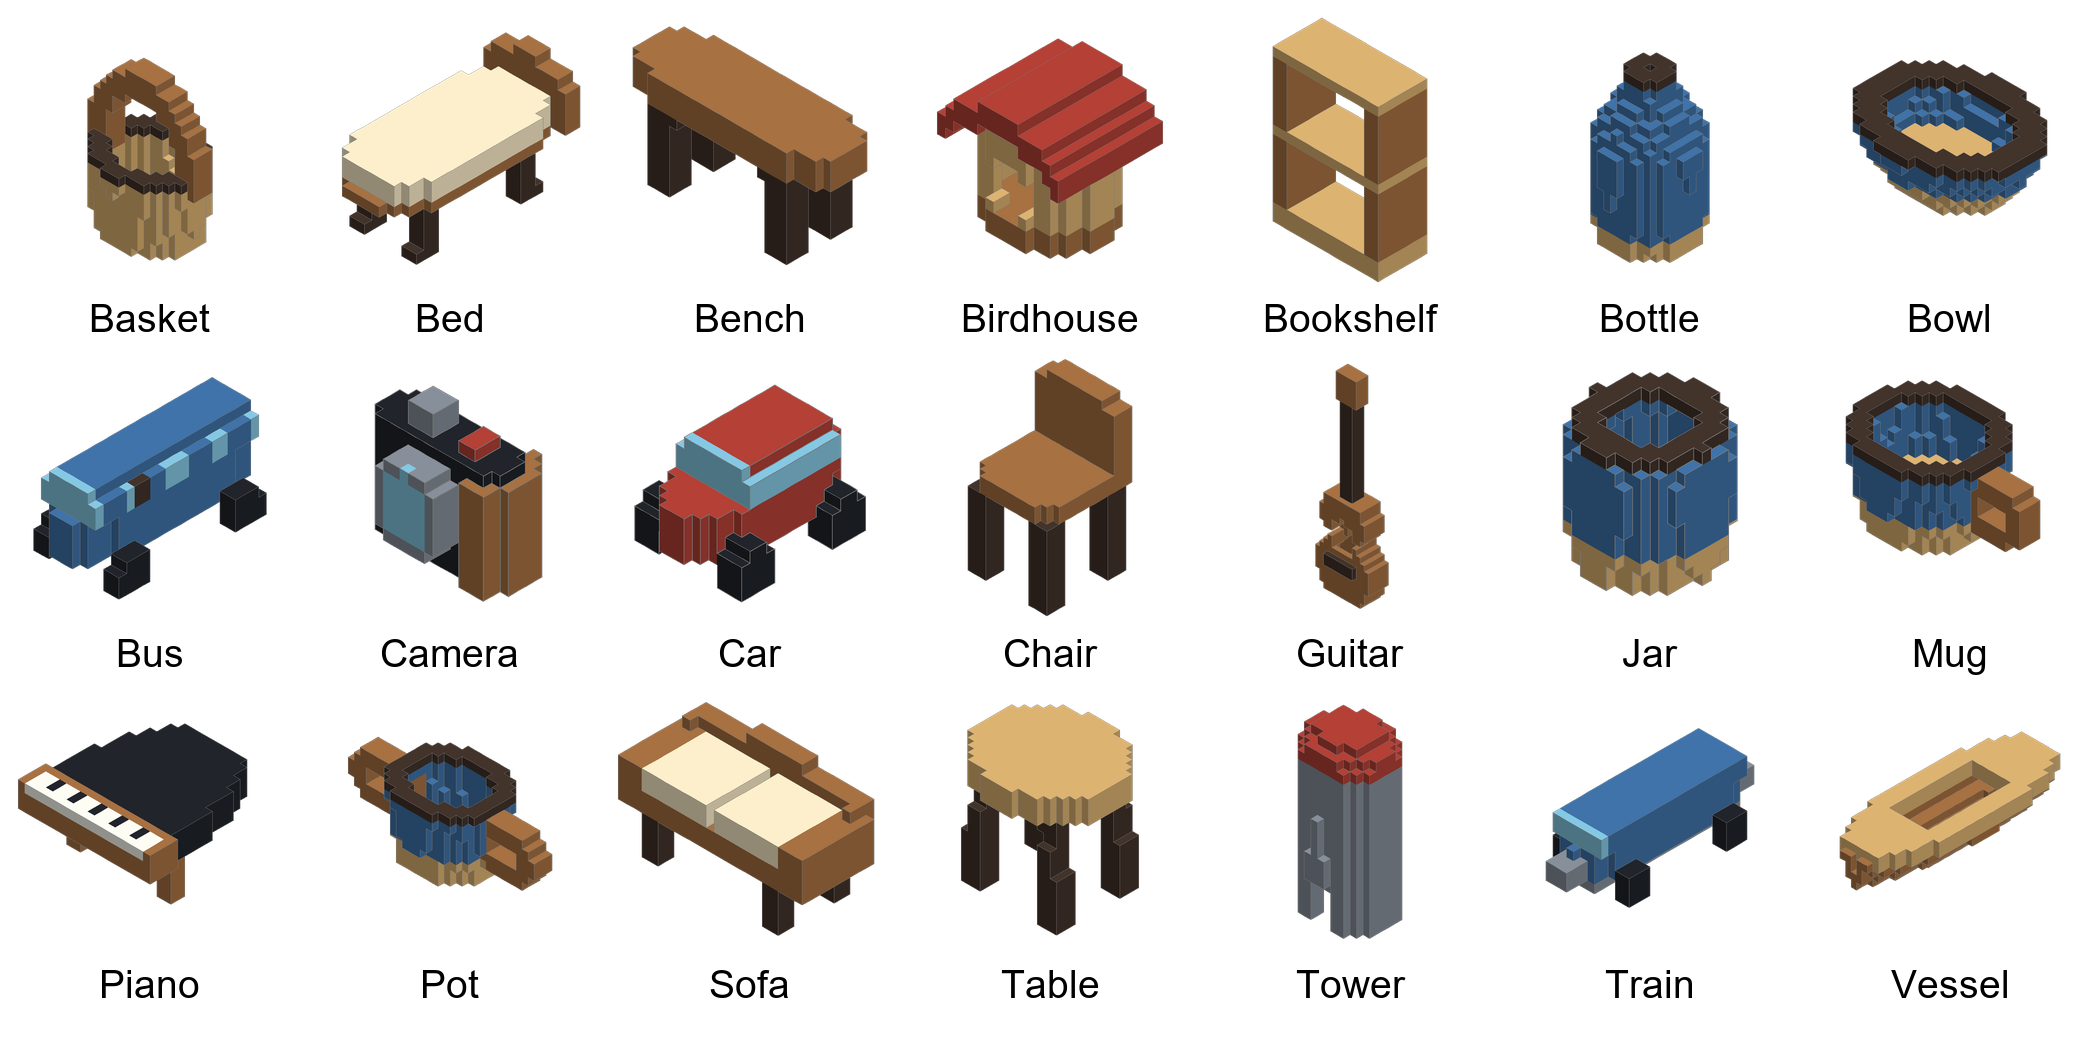
\includegraphics[width=\textwidth]{figures/image7_en.png}
\caption{Voxel model samples from the 21 object categories.}
\end{figure*}

\begin{figure*}[t]
\centering
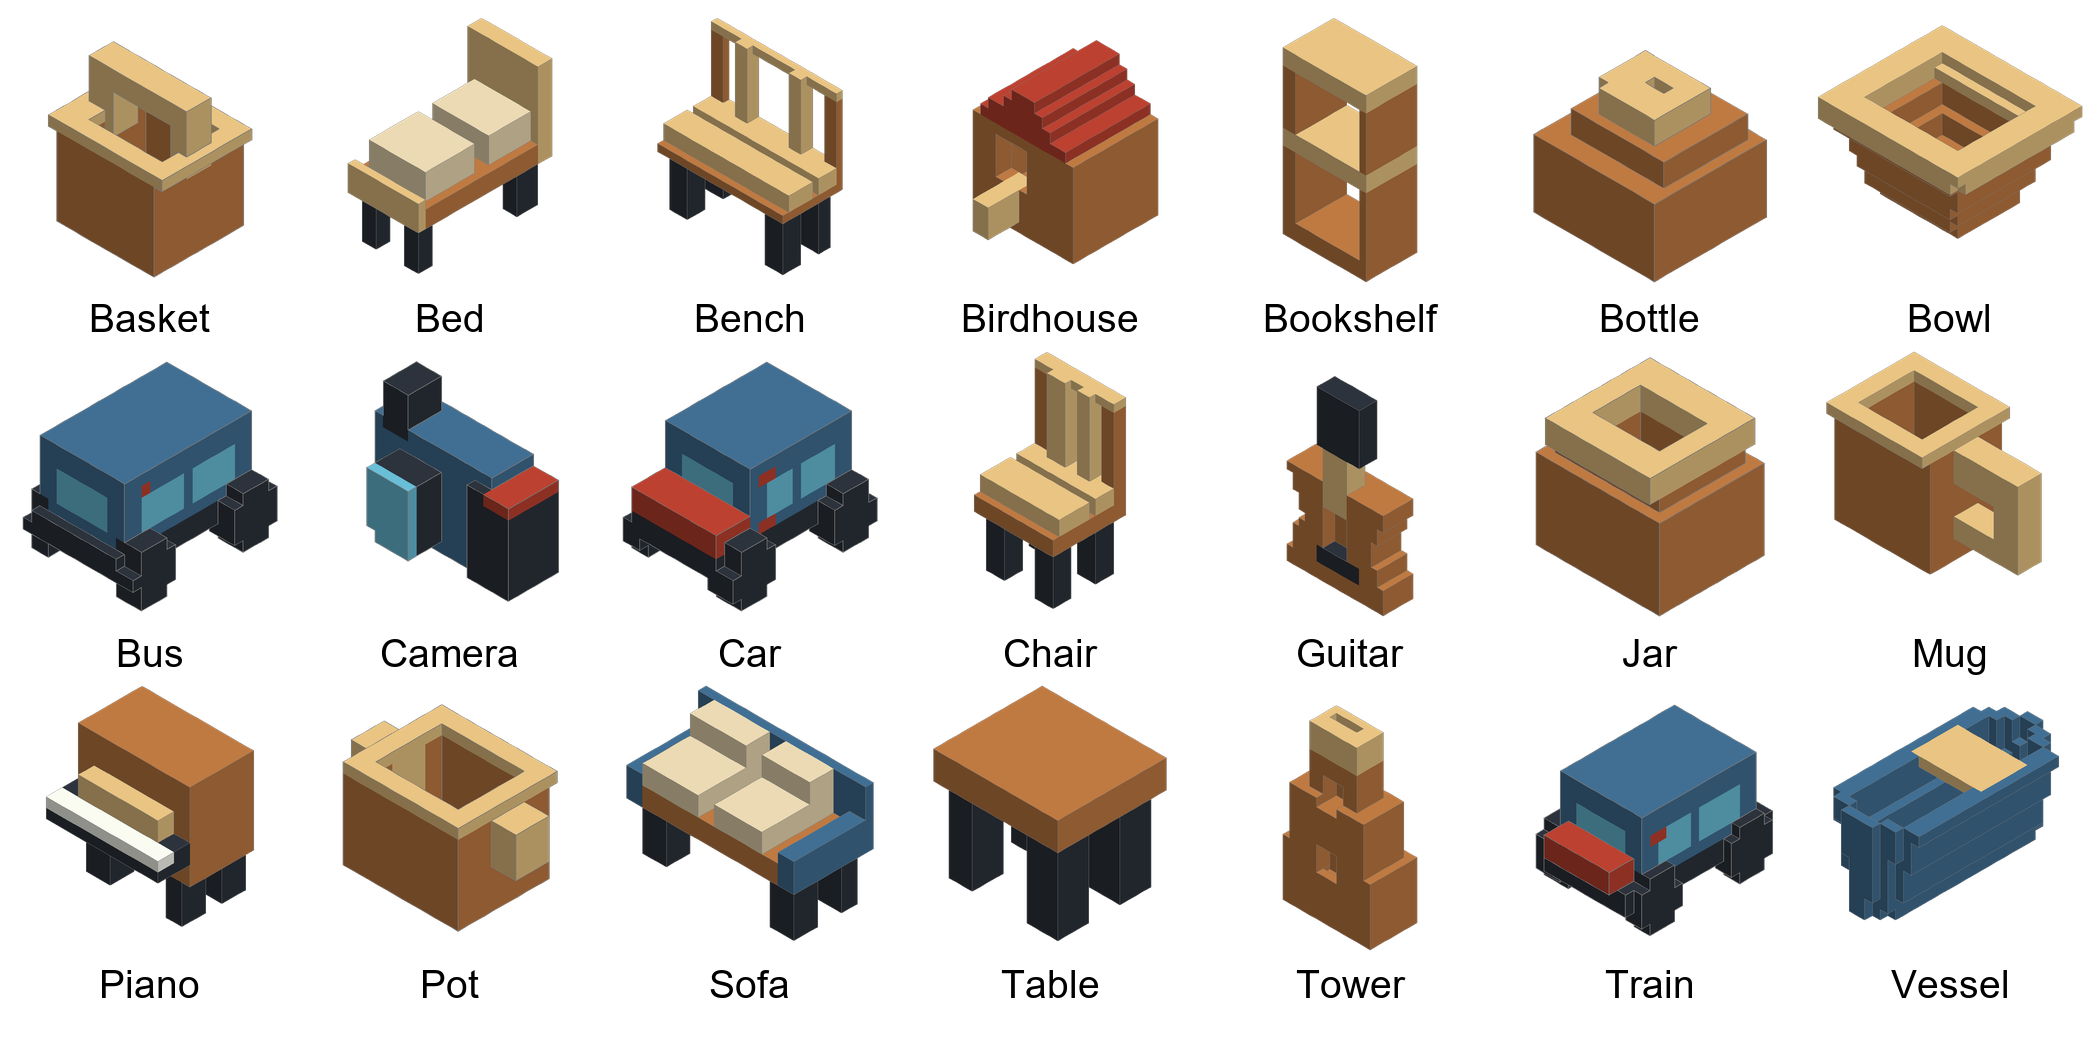
\includegraphics[width=\textwidth]{figures/image8_en.png}
\caption{Additional voxel model examples from an earlier release.}
\end{figure*}

\begin{figure*}[!htbp]
\centering
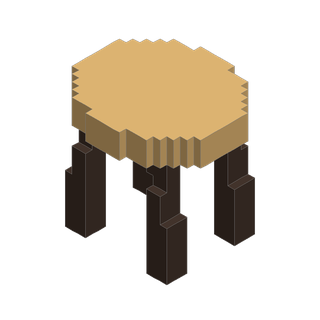
\includegraphics[width=0.118\textwidth]{figures/image4.png}\hfill
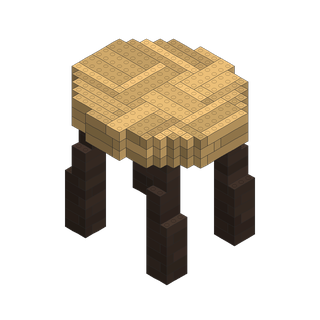
\includegraphics[width=0.118\textwidth]{figures/image5.png}\hfill
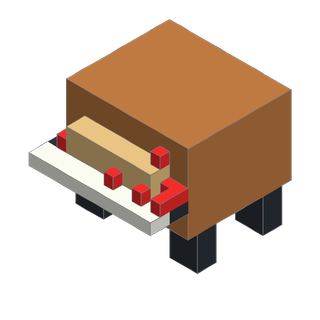
\includegraphics[width=0.118\textwidth]{figures/image2.png}\hfill
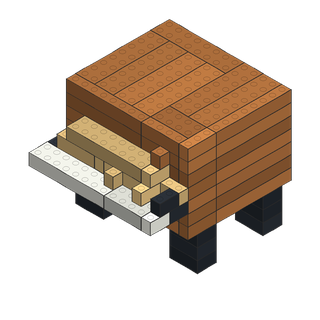
\includegraphics[width=0.118\textwidth]{figures/image3.png}\hfill
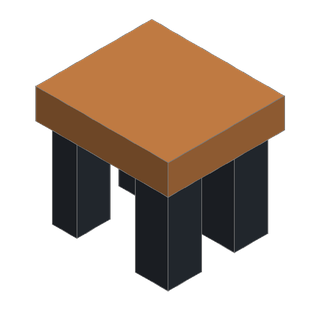
\includegraphics[width=0.118\textwidth]{figures/image9.png}\hfill
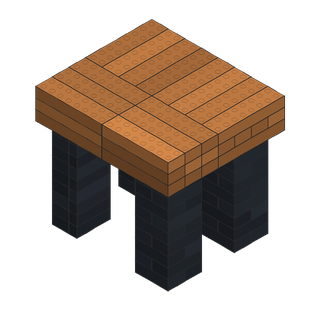
\includegraphics[width=0.118\textwidth]{figures/image10.png}\hfill
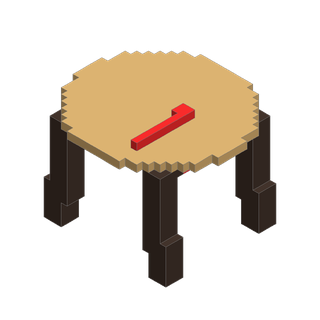
\includegraphics[width=0.118\textwidth]{figures/image11.png}\hfill
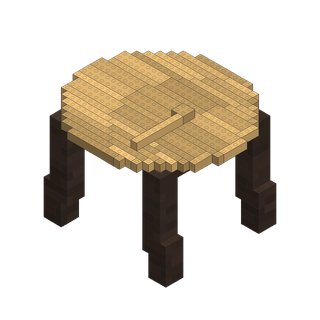
\includegraphics[width=0.118\textwidth]{figures/image12.png}
\caption{Examples of voxel targets and brick layouts after local repair, from an earlier release.}
\end{figure*}

\begin{figure*}[t]
\centering
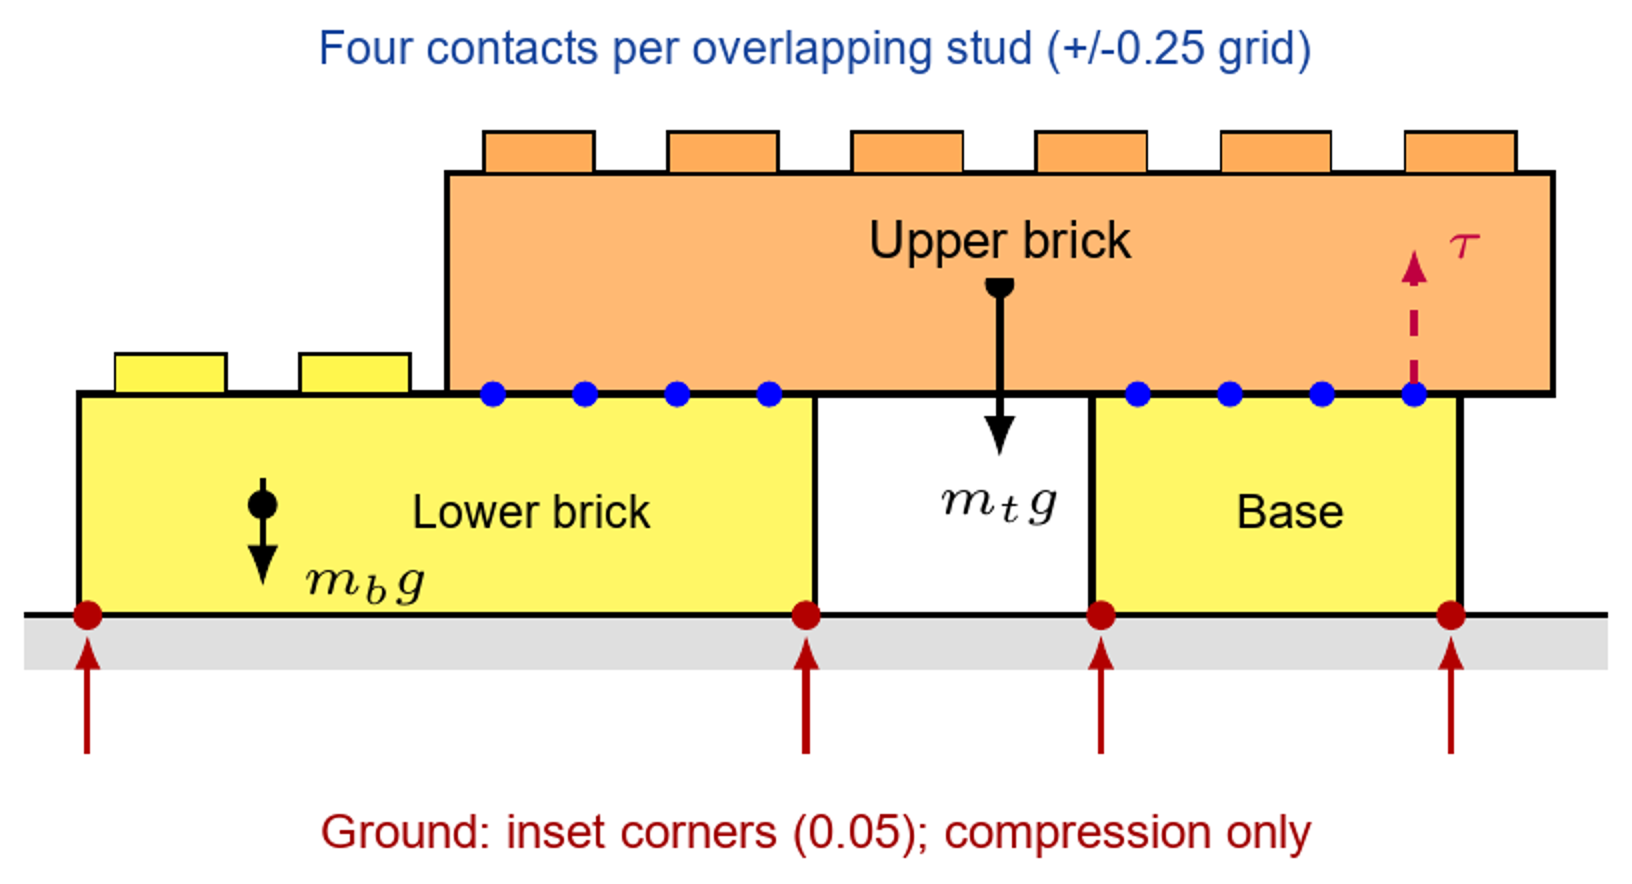
\includegraphics[width=0.75\textwidth]{figures/image13_en.png}
\caption{Contact-based gravity screening model from an earlier release, with English labels. The contact and ground assumptions are as stated above.}
\end{figure*}

\begin{figure*}[!htbp]
\centering
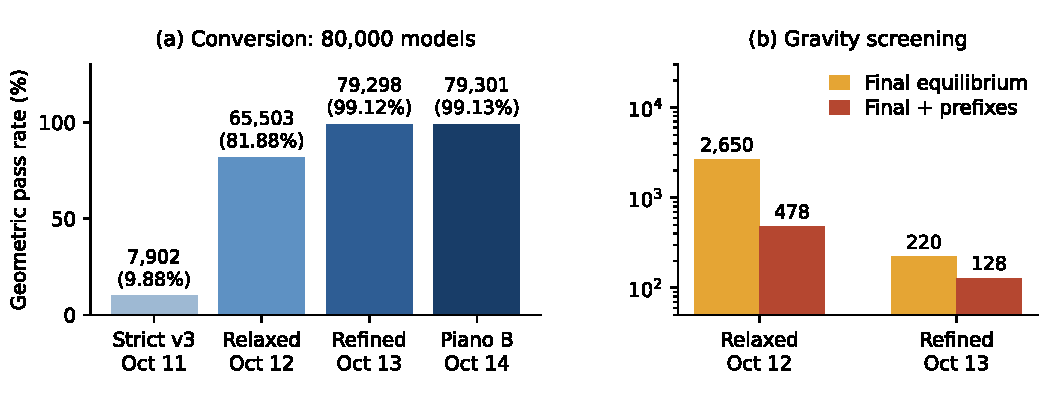
\includegraphics[width=\textwidth]{figures/image14_en.pdf}
\caption{Geometric conversion and screening outcomes across earlier releases; values as given in the corresponding release reports (Table~\ref{tab:conversion}).}
\end{figure*}

\begin{figure*}[!htbp]
\centering
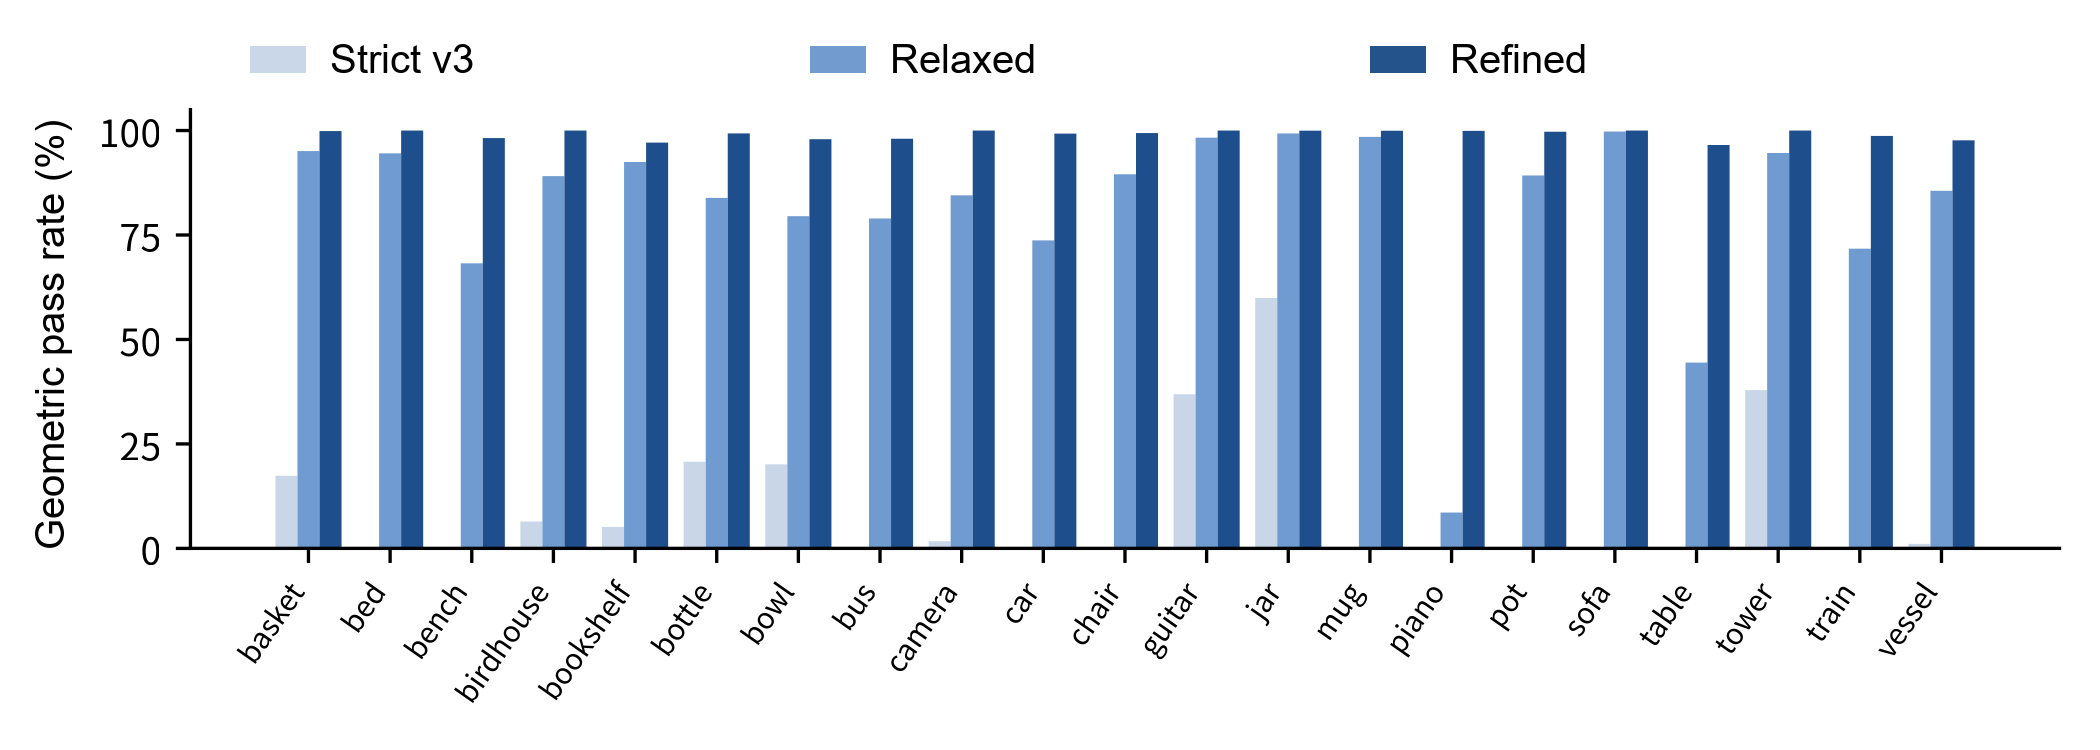
\includegraphics[width=\textwidth]{figures/image15_en.png}
\caption{Geometric pass rates by category for the three conversion releases in Table~\ref{tab:conversion}.}
\end{figure*}

\begin{figure*}[t]
\centering
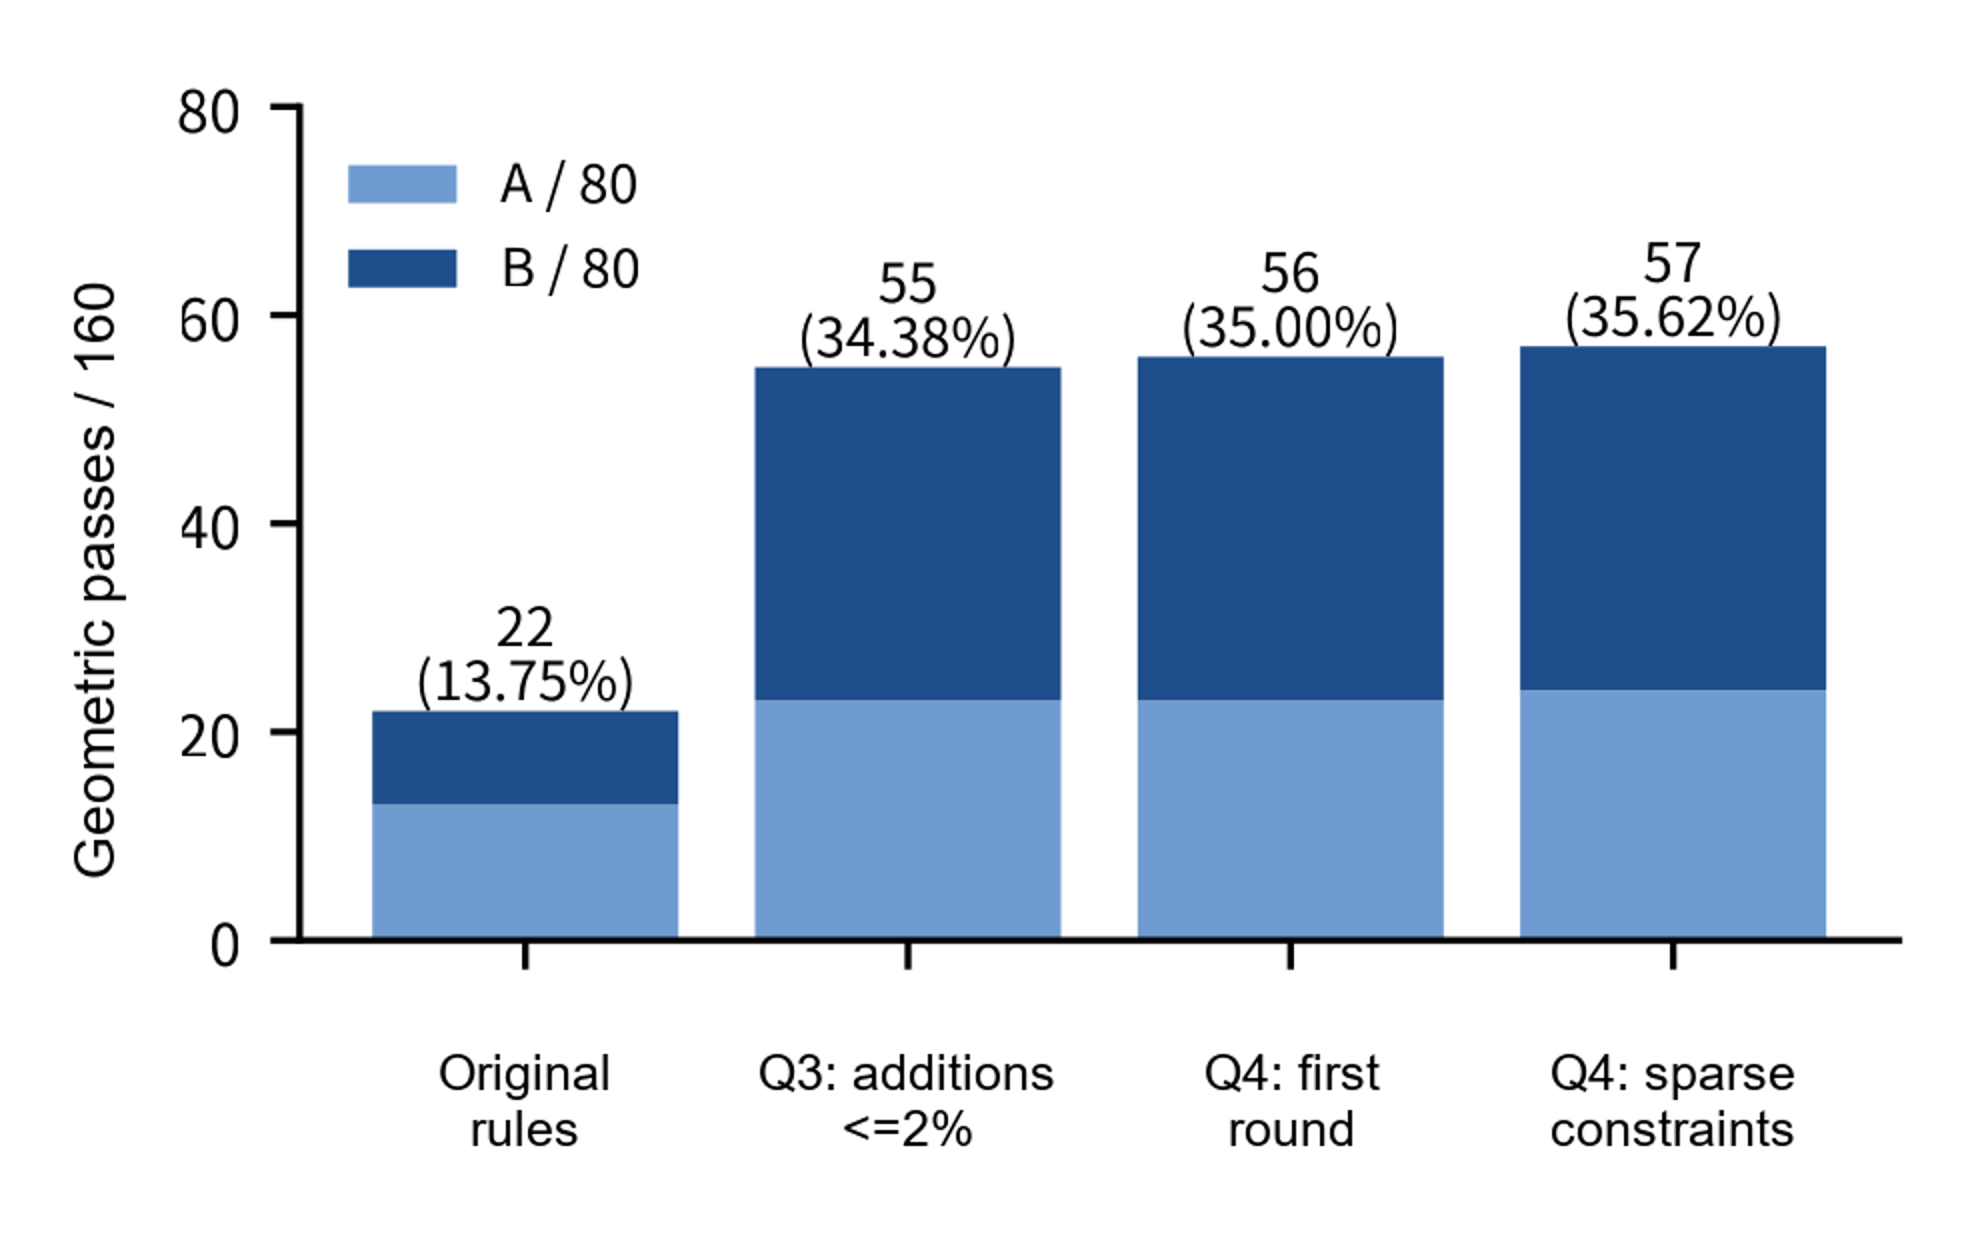
\includegraphics[width=0.72\textwidth]{figures/image16_en.png}
\caption{Geometric pass counts for the original rules, Q3, and two Q4 variants on the same 160-model sample (seed 38177). The Q4 rounds reuse this sample for tuning.}
\end{figure*}

\begin{figure*}[!htbp]
\centering
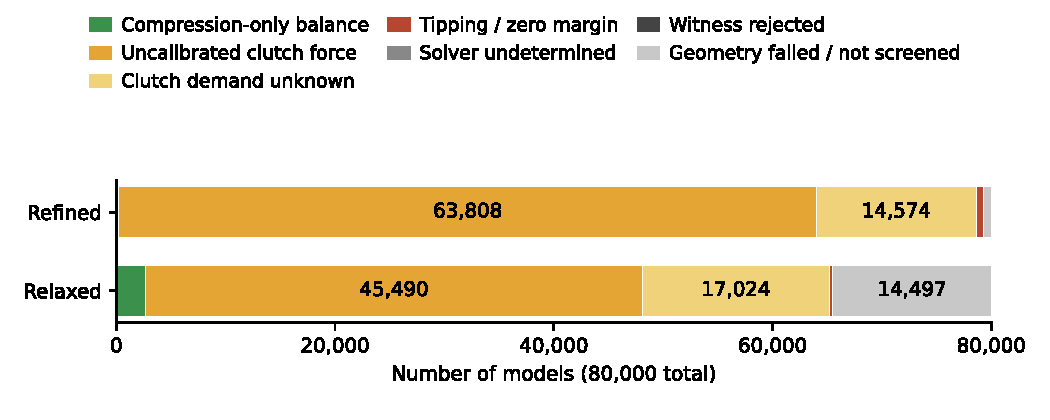
\includegraphics[width=\textwidth]{figures/image17_en.pdf}
\caption{Distributions of physical screening statuses in earlier releases; values as given in the corresponding release reports. Counts refer only to the releases shown and are reported separately from geometric pass rates.}
\end{figure*}


% Polished Appendix B: Training Details (proofread by Claude). Original text is in main-original.tex.
\section{Technical Appendix: Training Details}
\label{app:training}
Aggregate throughput is 24,448 tokens/s over eight GPUs, and the mean training loss is 0.0273. Evaluation and checkpointing run every 500 steps. With TRL~0.15, the unpacked multi-GPU path hangs after the first backward pass, so we pin the TRL~0.17 stack. Because validation loss is lowest during epoch 2, two epochs would be a more economical setting for future runs, saving about one third of the compute. The full software stack is transformers 4.51.3, trl 0.17.0, peft 0.15.2, datasets 3.6.0, and accelerate 1.6.0, with bf16 precision, gradient checkpointing, and unpacked sequences.

\begin{table}[!htbp]
\centering
\small
\begin{tabular}{lrr}
\toprule
Progress & Step & Validation loss \\
\midrule
Start & 500 & 0.1410 \\
--- & 1,500 & 0.0950 \\
--- & 10,500 & 0.0509 \\
--- & 22,500 & 0.0404 \\
$\approx$ End of epoch 1 & 44,500 & 0.0337 \\
--- & 65,500 & 0.0316 \\
Best (epoch 1.77) & 79,000 & 0.0308 \\
End of epoch 3 & 133,860 & 0.0339 \\
\bottomrule
\end{tabular}
\caption{Validation loss on the 2,000-sample validation subset. One epoch is $\approx$44,620 steps; step 44,500 is the evaluation closest to the end of epoch 1.}
\label{tab:eval-loss}
\end{table}

% BrickGPT-paper column verified against arXiv:2505.05469 (Sec. 5.1 and Appendix A training details).
\begin{table*}[!htbp]
\centering
\small
\setlength{\tabcolsep}{5pt}
\begin{tabular}{lcc}
\toprule
Dimension & BrickGPT paper & Official Qwen3 script (ours) \\
\midrule
Base model & LLaMA-3.2-1B-Instruct & Qwen3-1.7B \\
LoRA & $r=32$, $\alpha=16$, dropout $0.05$, $q$/$v$ only (3.4M params) & $r=16$, $\alpha=32$, all linear layers \\
Learning rate & $2{\times}10^{-3}$ (AdamW) & $10^{-4}$ \\
Effective batch & 64 & 8 \\
Max length & 4,096 & 8,192 \\
Epochs & 3 & 3 \\
Hardware & 8$\times$RTX A6000, 12\,h & 8$\times$4090D, 25.3\,h \\
Data & StableText2Brick, 47k structures / 240k prompts & BrickForma-48, 79.3k models / 396,610 samples \\
\bottomrule
\end{tabular}
\caption{Our configuration compared with the original BrickGPT paper~\cite{brickgpt}. BrickGPT values are taken from Sec.~5.1 and Appendix~A of arXiv:2505.05469: base model; LoRA with $r{=}32$, $\alpha{=}16$, dropout $0.05$, applied to $q$/$v$ only (3.4M parameters); AdamW with learning rate $0.002$; global batch 64; a 4,096-token length filter; 3 epochs; 8$\times$RTX A6000 for 12\,h; and 47k+ structures with 240k prompts. The data organization, instruction template, absence of thinking mode, and LoRA paradigm follow BrickGPT; the concrete hyperparameters follow the official Qwen3 adaptation, with the budget adjusted for the larger world, library, and corpus.}
\label{tab:brickgpt-recipe}
\end{table*}


% Polished Appendix C: Additional Evaluation Material (proofread by Claude). Original text is in main-original.tex.
\section{Technical Appendix: Additional Evaluation Material}
\label{app:eval}

\paragraph{Matched evaluation.}
The main comparison combines 525 final BrickForma exports with the 525 BrickGPT and 525 BrickNet exports scored in the original comparison. The final BrickForma run uses the same prompt IDs, captions, categories, and description levels as the raw run. Its manifest records 445 layouts refined from the original drafts, 34 originals retained, and 46 regenerated layouts. The retained layouts reproduce all three original alignment scores exactly. The manifest records voxel removals in two cases (72 for \texttt{A14\_L5} and 1,486 for \texttt{A34\_L2}). For all 525 final layouts we compute four metrics and render eight views per export (4,200 new views), yielding 1,575 scored exports and 12,600 views in the combined comparison. We compute $P_{\mathrm{inv}}$ on the final LDraw file order and report geometric connectivity separately on the diagnostic cohort below.

\paragraph{Raw export provenance.}
The raw comparison used 265 previously delivered Q8\_0 exports and 260 supplemental exports, with a single delivered raw BrickForma draft per prompt before refinement. The supplemental records flag 8 incomplete generations and 96 failures of the source geometry check among the 260 exports; the two sets may overlap. The 265 earlier exports have no corresponding completion or geometry flags. The raw comparison rendered the delivered LDraw sequences because three supplied GLB previews contained only a prefix of the assembly. BrickGPT uses a $20^3$ world and seed 42, with recorded regeneration budgets of 8 or 100. The 260 supplemental BrickForma exports were generated locally without MILP refinement, using checkpoint \texttt{BrickGPT-Qwen3-1.7B-BrickMore-48} (revision \texttt{92d1c595}) in \texttt{bfloat16} precision with \texttt{sdpa} attention, \texttt{max\_new\_tokens}=8192, \texttt{temperature}=0.7, \texttt{top\_p}=0.9, and the seed schedule $(42,104,2026)$, with zero overlap with the training set. The 265 earlier Q8\_0 exports come from an earlier inference batch whose per-sample decoding flags were not logged. Finally, the 105-sample difference between $79{,}301{\times}5=396{,}505$ and the 396,610 logged training pairs stems from a minor snapshot offset between the final dataset release and the training run.

\begin{samepage}
\paragraph{Baseline versions.} The archived 260-prompt BrickGPT runner is based on GitHub commit \texttt{9c53c7c} of \url{https://github.com/AvaLovelace1/BrickGPT}. Its generation report records a local checkpoint that combines \texttt{meta-llama/Llama-3.2-1B-Instruct} with the public \texttt{AvaLovelace/BrickGPT} LoRA adapter. The runner can load a premerged checkpoint or merge these weights through PEFT's \texttt{merge\_and\_unload}; the report identifies the merged checkpoint used, but no separate merge log exists. The BrickNet GitHub reference snapshot is commit \texttt{283faf7} of \url{https://github.com/kulits/BrickNet}, and the public 1.7B PT and SFT adapter revisions on \texttt{Qwen/Qwen3-1.7B} are \texttt{0f75d5e5} and \texttt{3fe7f4c1}, respectively. The other 265 BrickGPT exports and the BrickNet exports have no recorded generation-code commit. Invalid-placement scoring uses the inset collision kernel from the pinned \texttt{bricknet==0.1.0} PyPI wheel.

\paragraph{Reference dataset snapshots.} BrickGPT uses StableText2Brick (public data upload \texttt{1dcf904} at \texttt{AvaLovelace/StableText2Brick}). BrickNet uses the gated PT, SFT, and validation splits described in \texttt{DATA.md} at GitHub commit \texttt{283faf7}; the release documentation identifies these splits by file name and gives no separate dataset revision.
\end{samepage}

\paragraph{Untuned Qwen3-1.7B.} None of the 260 untuned outputs passed the generation-time geometry check. The strict parser found no placements in 178 outputs, and two more used an unsupported part type. We assign these 180 outputs zero VQAScore, PE, and SigLIP2, and keep the measured scores for the 80 scorable partial layouts, so all alignment means are over the same 260 prompts. On the 80 pairs with scorable base layouts, the mean file-order invalid-placement ratio is 39.67\% for the untuned model and 1.01\% for raw BrickForma. The comparison applies common scoring to delivered generation runs whose decoding settings may differ.

\paragraph{Paired tests and truncation.}
Table~\ref{tab:sig} compares final BrickForma outputs with each baseline on the 525 prompts. We use a two-sided exact sign test and a two-sided Wilcoxon signed-rank test with the normal approximation, excluding ties, and apply Holm correction separately to the six comparisons within each test. All adjusted $p$ values are below $5.0{\times}10^{-8}$. PE truncates 121 prompts and SigLIP2 truncates 209. On the untruncated subsets, BrickForma, BrickGPT, and BrickNet score 0.1523, 0.1408, and 0.1135 on PE (404 prompts) and 0.0339, 0.0157, and 0.0009 on SigLIP2 (316 prompts).

\begin{table}[t]
\centering\small
\setlength{\tabcolsep}{3pt}
\begin{tabular}{llrrr}
\toprule
Baseline & Metric & W/L/T & Sign $p_H$ & Wilc.\ $p_H$ \\
\midrule
BrickGPT & VQAScore & 372/153/0 & $1.4\times 10^{-21}$ & $5.6\times 10^{-19}$ \\
 & PE & 341/184/0 & $1.4\times 10^{-11}$ & $1.0\times 10^{-13}$ \\
 & SigLIP2 & 323/198/4 & $4.8\times 10^{-8}$ & $1.0\times 10^{-12}$ \\
BrickNet & VQAScore & 456/69/0 & $3.4\times 10^{-70}$ & $2.1\times 10^{-60}$ \\
 & PE & 417/108/0 & $4.0\times 10^{-43}$ & $9.3\times 10^{-51}$ \\
 & SigLIP2 & 410/113/2 & $5.9\times 10^{-40}$ & $1.3\times 10^{-43}$ \\
\bottomrule
\end{tabular}
\caption{Two-sided paired tests for final BrickForma outputs on 525 prompts. W/L/T counts BrickForma wins, losses, and ties. Each test applies Holm correction across its six comparisons.}
\label{tab:sig}
\end{table}


\paragraph{Earlier 114-prompt comparison.} BrickGPT outputs were generated in its native $20^3$ world (seed 42), whereas BrickForma places bricks in a $48^3$ workspace, which partly explains the difference in part counts. The systems also differ in candidate selection, filtering, and post-processing. On the BrickForma side, 45 of the 114 comparison outputs, together with their prompts, were chosen by human review as the best of six candidate phrasings in a category--level group; a winner was found in 79 of the 105 groups, and 45 of those winners entered this comparison. The remaining 69 outputs come from later fill-in, regeneration, collaborator, and review rounds: 35 replaced a judged winner in 34 groups, and 34 filled 26 groups in which no candidate had been judged acceptable. Together, the 114 outputs cover all 105 groups.\footnote{The six candidates are the five new-batch phrasings and one first-batch phrasing documented in the evaluation-set README. Of the 69 later outputs, 21 come from a review round, 16 and 7 from two collaborator-contributed sets, 12 from a second-round redo, 7 from a third-round fill-in, 5 from regeneration, and 1 from a car-specific trial, as recorded in the delivery manifest. BrickGPT was then run once on each selected prompt (seed 42), and BrickNet contributed one accepted sample per prompt (up to 30 attempts).} The 114 outputs comprise 110 refined layouts and four raw layouts. The earlier BrickGPT records report an eight-regeneration budget with Gurobi disabled.

\paragraph{Sensitivity of the earlier comparison.}
With equal weighting over the 105 category--level groups, BrickForma scores 0.2347, 0.1840, and 0.1257 and BrickGPT scores 0.1511, 0.1459, and 0.0318 on VQAScore, PE, and SigLIP2, respectively. After excluding prompts truncated by each encoder, PE is 0.1821 versus 0.1445 on 89 prompts, and SigLIP2 is 0.1088 versus 0.0301 on 85 prompts. The PE and SigLIP2 text encoders read at most 72 and 64 tokens, respectively.

\paragraph{Inference refinement.}
For the clipped voxel union $C$, let $\mathcal{B}(v)$ index the candidate placements from the oriented footprint library that cover $v$ and lie entirely within $C$. With binary placement variables $x_b$, exact coverage requires $\sum_{b\in\mathcal{B}(v)}x_b=1$ for each $v\in C$, which preserves the union and excludes overlaps. To enforce a single stud-connected component, a standard single-commodity flow formulation routes flow from a virtual root $r$ through directed stud-contact edges $(b,b')\in\mathcal{E}$ between adjacent layers. Grounded candidate placements $b\in\mathcal{B}_{\mathrm{gnd}}$ receive root inflow $f_{r,b}\ge 0$; internal edge flows satisfy $0\le f_{b,b'}\le M x_b$ and $0\le f_{b,b'}\le M x_{b'}$ with capacity bound $M=|C|$; and flow conservation $\sum_{(u,b)\in\mathcal{E}\cup\{(r,b)\}} f_{u,b} - \sum_{(b,v)\in\mathcal{E}} f_{b,v} = x_b$ ensures that every selected placement is connected to the root. We solve the MILP with SciPy's HiGHS interface under the time tiers of Algorithm~\ref{alg:inference-refinement}, and a feasible cover must also pass the independent placement, coverage, and connectivity audit. The logged run summaries record the solver time tiers and audit outcomes, but per-run objective weights and gap tolerances were not retained. Contact-based self-weight screening uses a separate LP (Appendix~\ref{app:dataset}).

\paragraph{Separate diagnostic cohort.}
We inspected 525 other BrickForma generations in a structural diagnostic (21 categories $\times$ five levels $\times$ five phrasings). Together with 105 first-batch prompts, this diagnostic batch formed the six-phrasing candidate pool from which 45 of the 114 comparison outputs were selected (35 of them from the 525), as described above. Algorithm~\ref{alg:inference-refinement} describes the default candidate-selection and refinement rules. The diagnostic manifests record either a refinement tier or a raw layout kept unchanged. For 28 prompts, a recovery path sampled seeds outside $S$; for two further prompts, the solver budget was extended to 600\,s. Only 46 raw layouts (8.8\%) form a single stud-connected component without refinement. This rate shows no clear trend across levels (13, 9, 9, 7, and 8 for L1--L5) but varies strongly by category (e.g., 8/25 for sofa and 0/25 for basket and camera). All 479 failing raw layouts split into at least two stud components (median 5, maximum 33). Overlaps are a minor cause: 50 failing layouts contain duplicated voxels, 41 of them at most five (median 2), and 429 contain none. The 2,240 detached fragments are mostly airborne (1,320 airborne versus 920 grounded). The learned model thus places bricks whose in-bounds voxel union is retained by refinement but that often fail to interlock across layers; all 525 final assemblies form a single stud-connected component with that union unchanged (Table~\ref{tab:diag}). These checks evaluate stud connectivity and consistency of the in-bounds voxel union, not prompt-level shape fidelity or spatial reasoning.

\begin{figure*}[t]
\centering
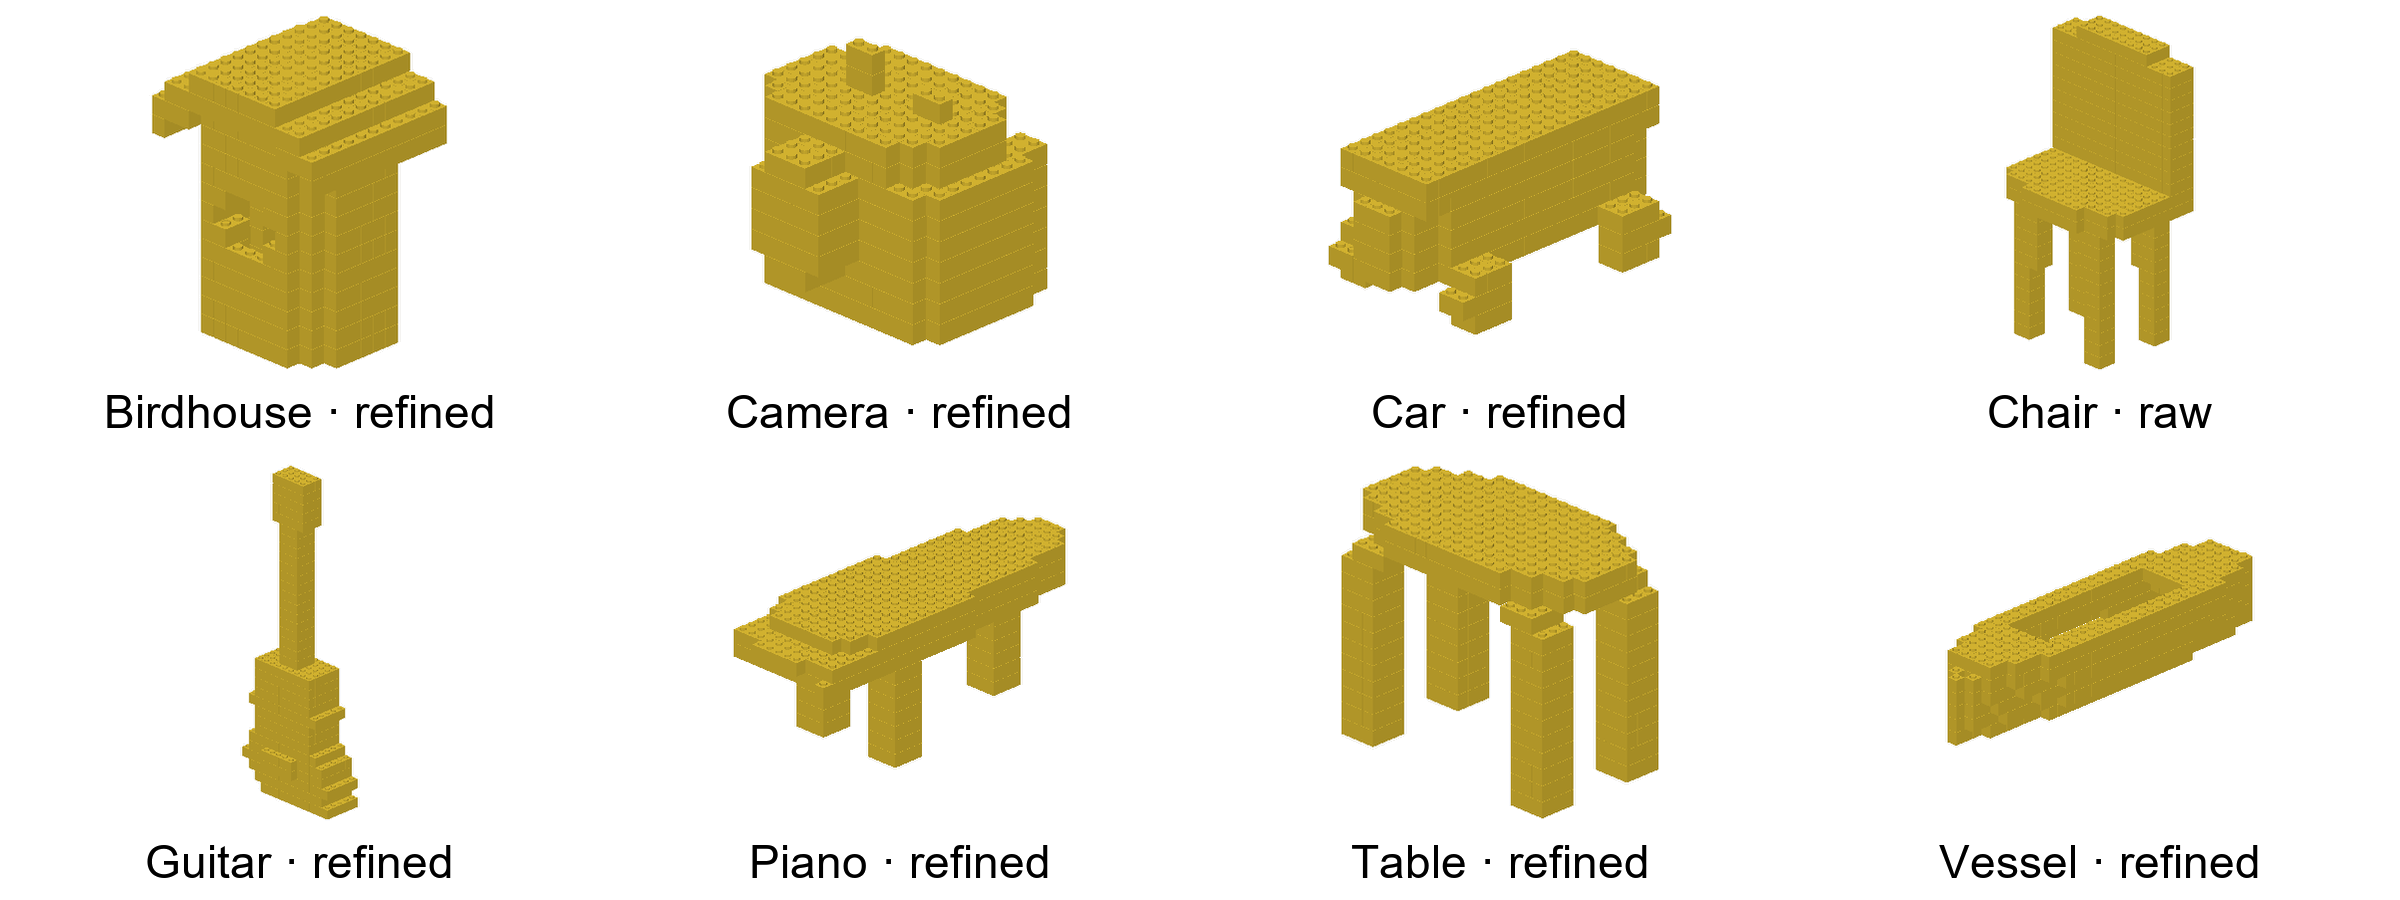
\includegraphics[width=\textwidth]{figures/generated_gallery_en.png}
\caption{BrickForma outputs from the earlier 114-prompt comparison. The chair is raw; the other examples are refined.}
\end{figure*}

\begin{table*}[!htbp]
\centering
\small
\setlength{\tabcolsep}{3pt}
\begin{tabular}{lr}
\toprule
Quantity (525 prompts) & Value \\
\midrule
Raw layout is a single stud component & 46 (8.8\%) \\
Stud components per failing raw layout (median / max) & 5 / 33 \\
Failing raw layouts with duplicated voxels & 50 / 479 \\
Detached fragments (airborne / grounded) & 1,320 / 920 \\
MILP tier reached (12 / 60 / 180 / 600\,s) & 326 / 133 / 18 / 2 \\
Prompts resampled outside $S$ & 28 \\
Final: single stud component, union unchanged & 525 / 525 \\
Raw bricks, median (range) & 183 (77--623) \\
Final assembly bricks, median & 452 \\
\bottomrule
\end{tabular}
\caption{Structural diagnostics on the separate 525-prompt cohort (Section~\ref{sec:diagnostics}). ``Union unchanged'' means that the final assembly covers exactly the in-bounds voxel union of the raw draft; it does not assess whether the shape matches the prompt.}
\label{tab:diag}
\end{table*}

\begin{figure*}[!htbp]
\centering
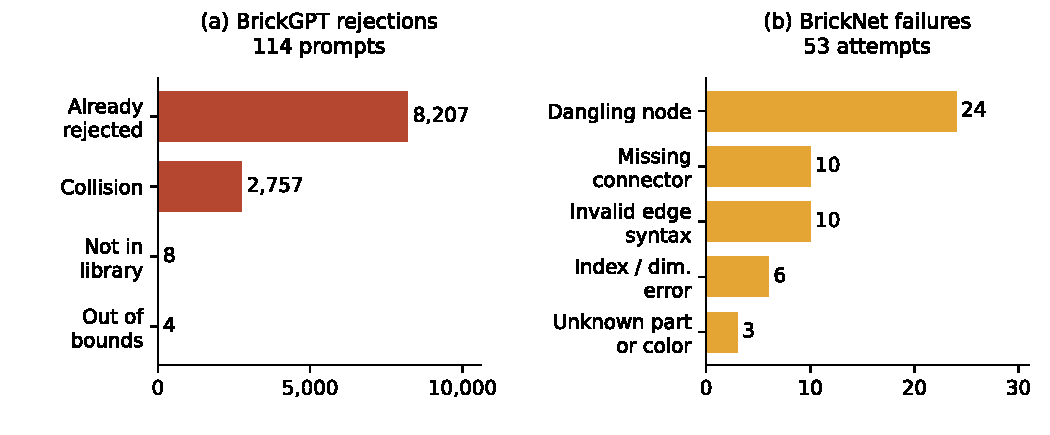
\includegraphics[width=\textwidth]{figures/image19_en.pdf}
\caption{Failure categories in the earlier 114-prompt comparison; values as given in the corresponding run records.}
\end{figure*}

\begin{figure*}[!htbp]
\centering
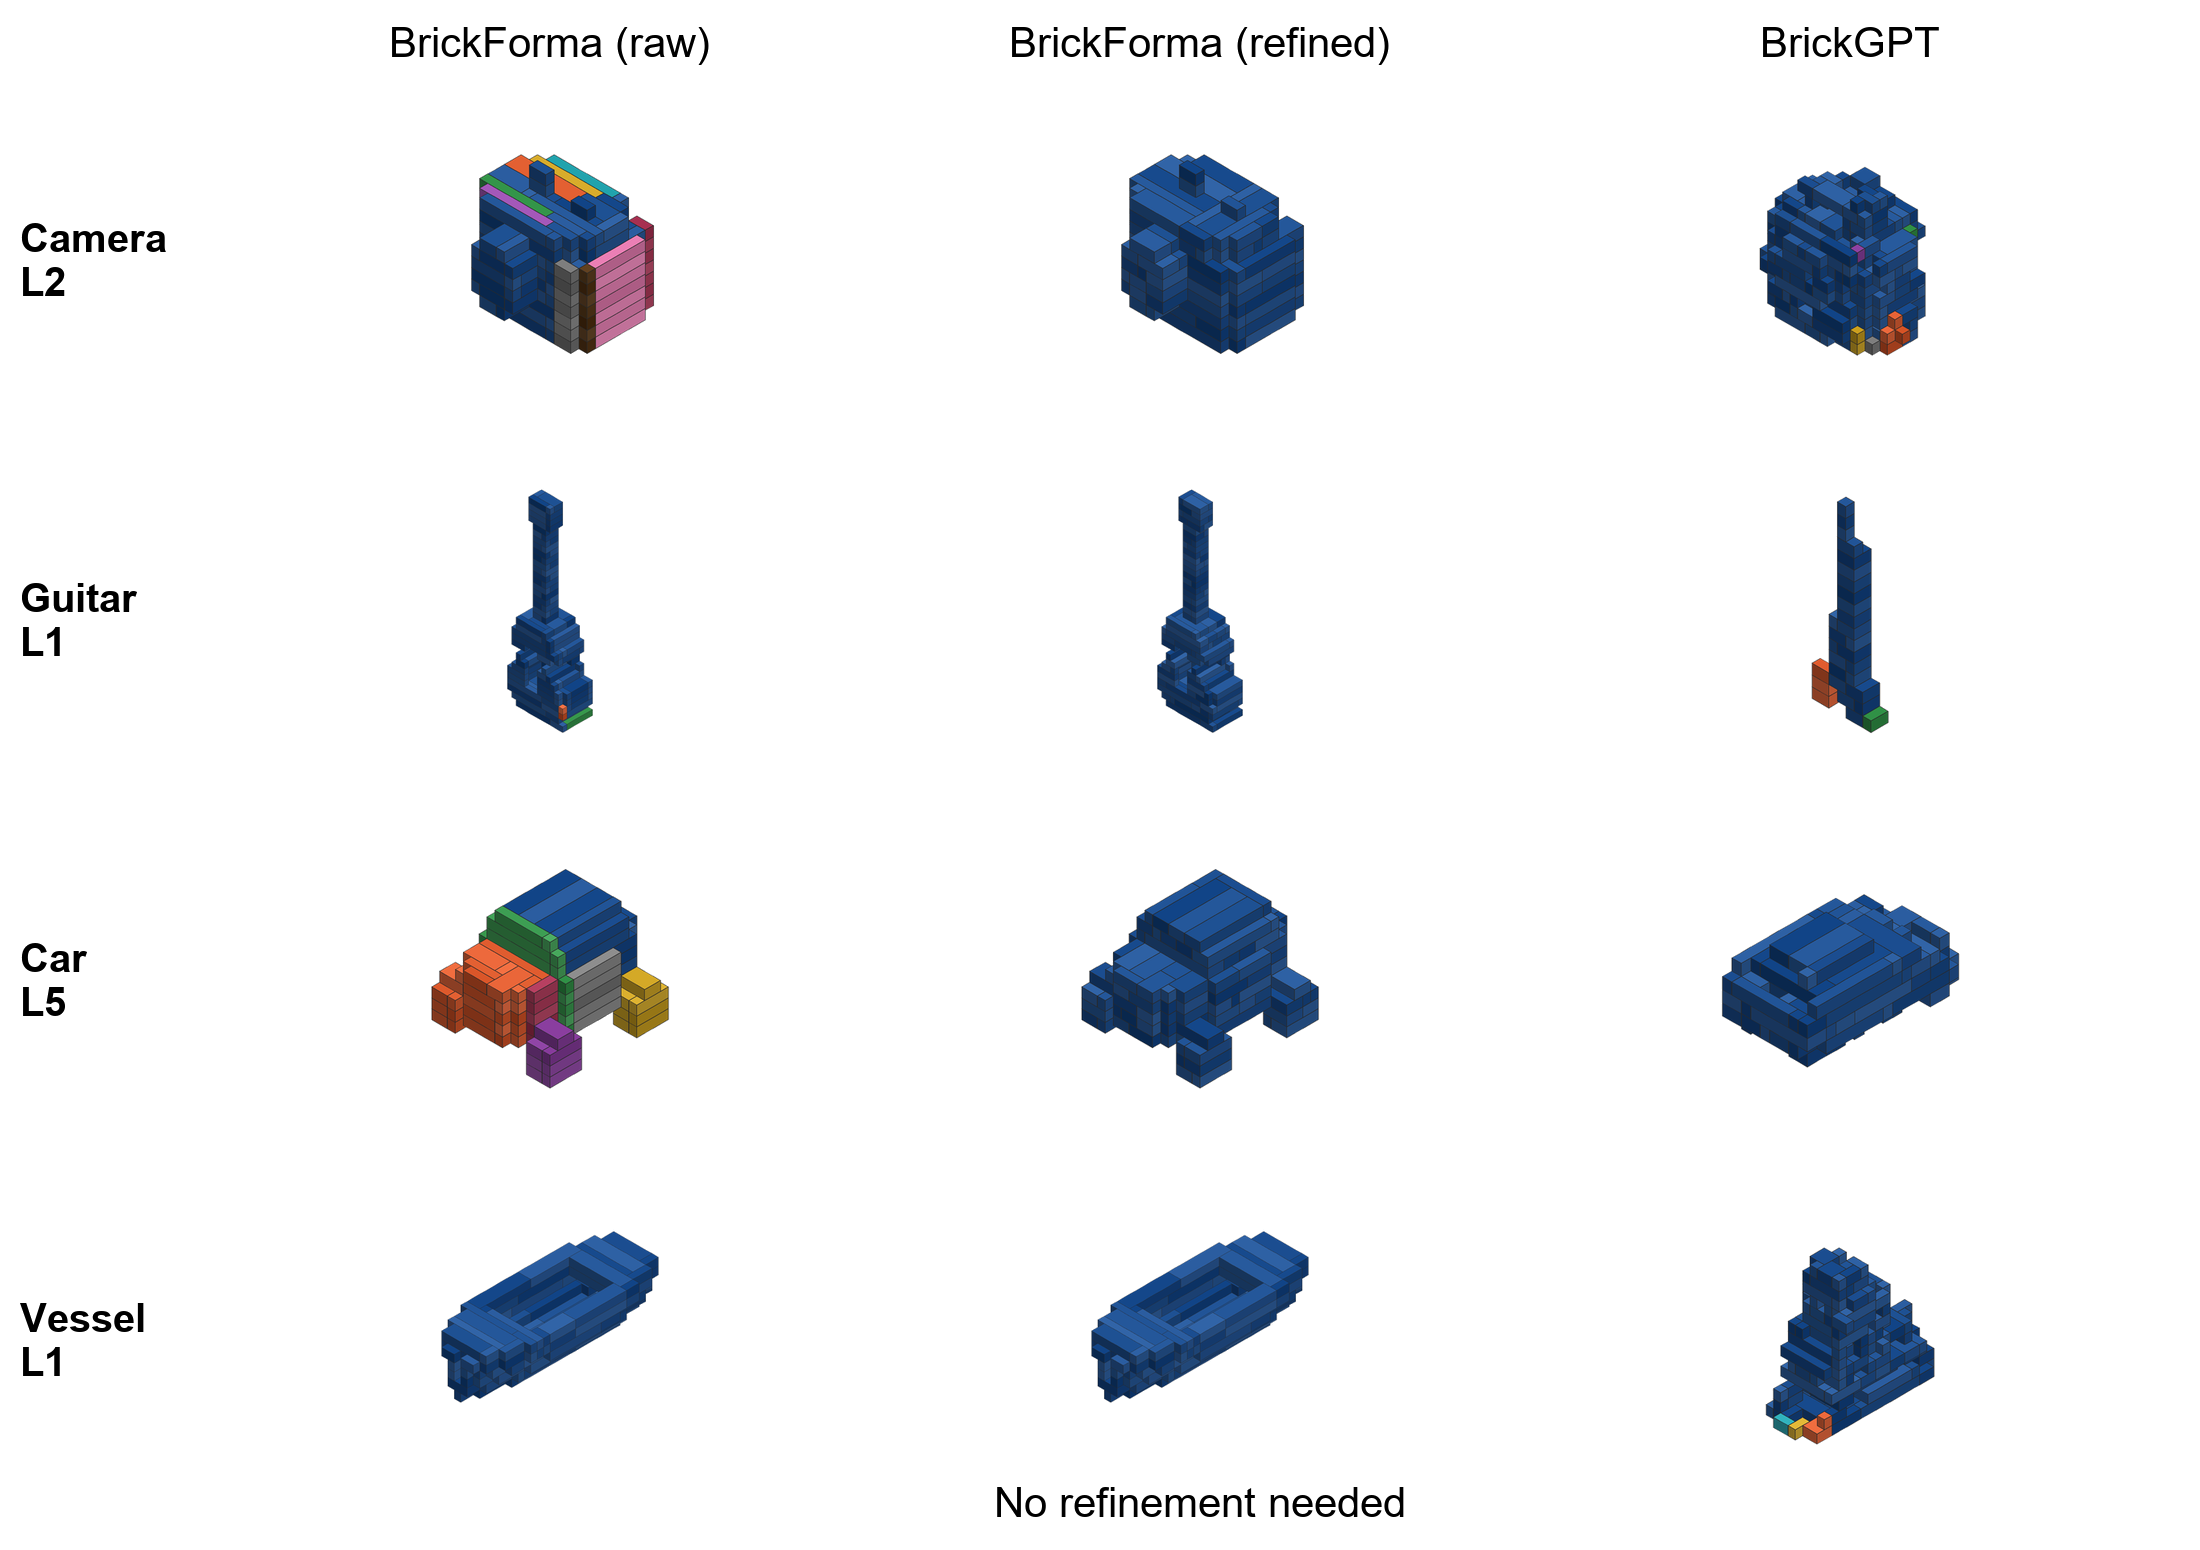
\includegraphics[width=\textwidth]{figures/original_comparison_en.png}
\caption{Qualitative examples from the earlier comparison. Columns show raw and refined BrickForma outputs and BrickGPT outputs.}
\end{figure*}

\begin{figure*}[t]
\centering
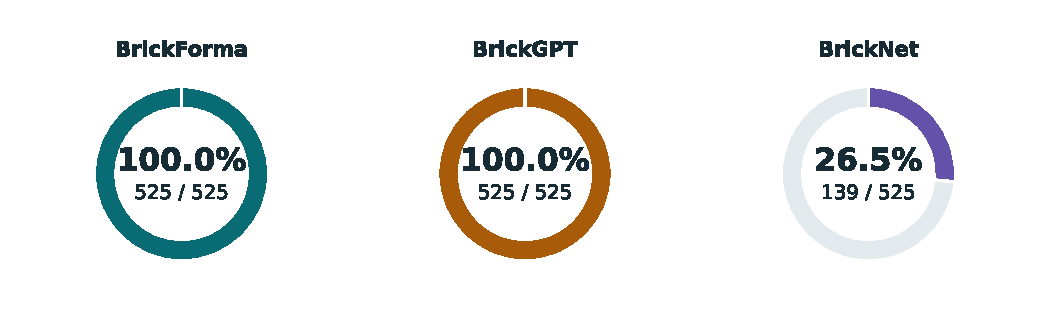
\includegraphics[width=\textwidth]{figures/comparison_20261119/01-zero-invalid.pdf}
\caption{Outputs with zero invalid placements on the 525 matched prompts. Colored arcs show outputs with $P_{\mathrm{inv}}=0$, and gray arcs show outputs with $P_{\mathrm{inv}}>0$. Each panel contains 525 outputs. BrickForma uses final outputs after refinement and recovery.}
\label{fig:comparison-zero-invalid}
\end{figure*}

\begin{figure*}[t]
\centering
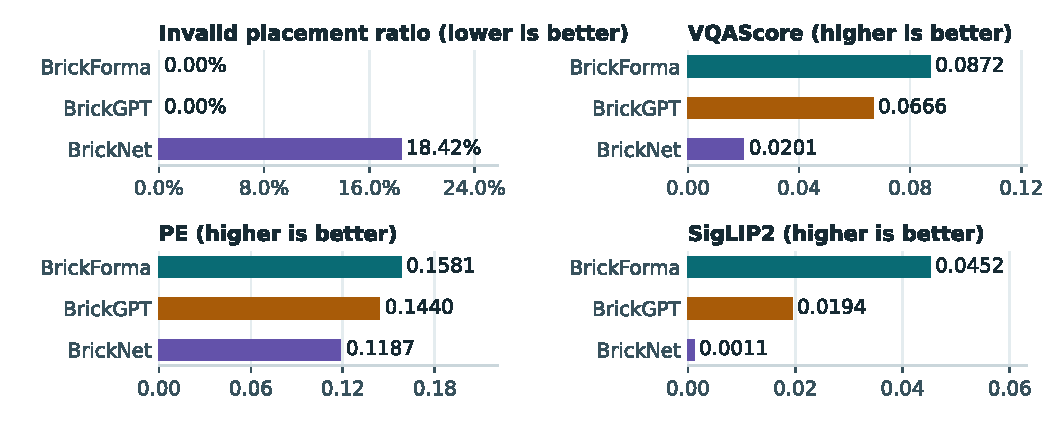
\includegraphics[width=\textwidth]{figures/comparison_20261119/02-means.pdf}
\caption{Mean scores on the 525 matched prompts. Each mean weights all prompts equally. The plotted values match Table~\ref{tab:main}.}
\label{fig:comparison-means}
\end{figure*}

\begin{figure*}[t]
\centering
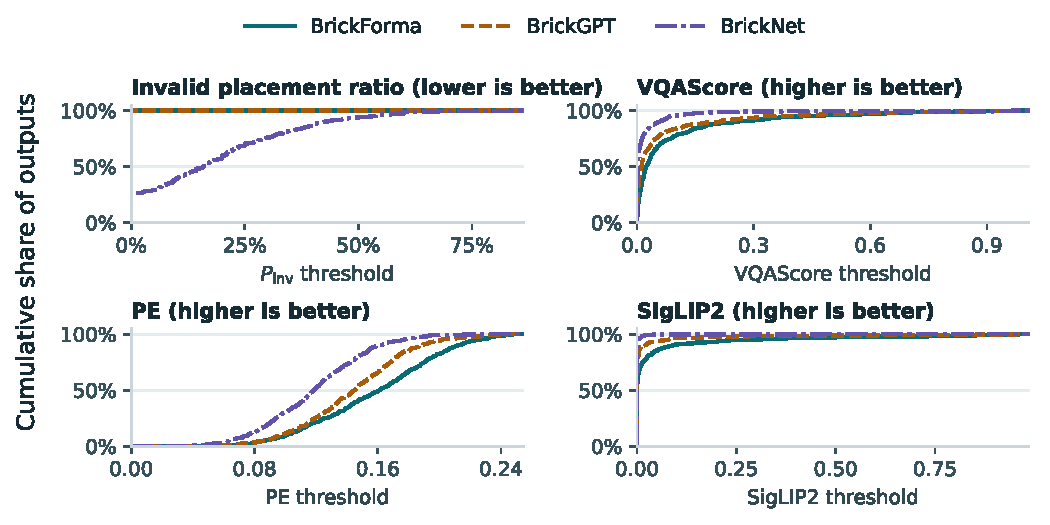
\includegraphics[width=\textwidth]{figures/comparison_20261119/03-distributions.pdf}
\caption{Empirical cumulative distributions of the four scores. Each curve gives the fraction of a system's 525 outputs that score at or below the threshold on the horizontal axis.}
\label{fig:comparison-distributions}
\end{figure*}

\begin{figure*}[t]
\centering
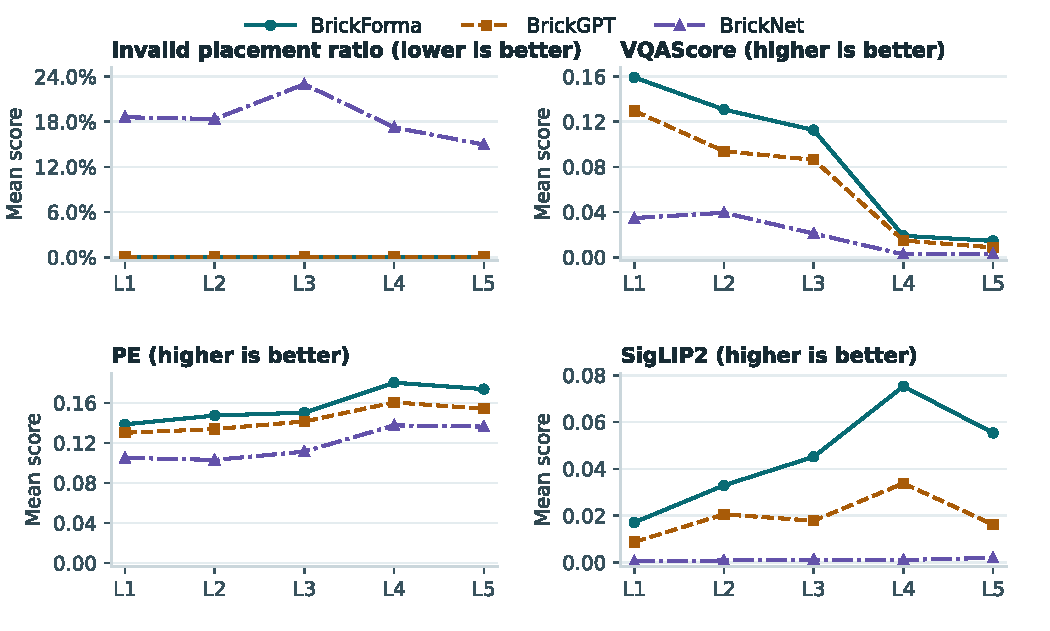
\includegraphics[width=\textwidth]{figures/comparison_20261119/04-by-level.pdf}
\caption{Mean scores from L1 to L5. Each point averages the 105 prompts shared by all three systems at that level (Table~\ref{tab:level-results}). From L3 to L4, VQAScore falls for all three systems, while PE rises.}
\label{fig:comparison-levels}
\end{figure*}



\FloatBarrier % keep Appendix C floats ahead of Appendix D
% Polished Appendix D: Historical Tables (proofread by Claude). Original text is in main-original.tex.
\section{Technical Appendix: Historical Tables}
\label{app:historical}
The following tables are transcribed from earlier project records. They use different versions or evaluation criteria and do not replace the main comparison. Where a value is superseded by a verified number in the main text (e.g., Table~\ref{tab:training-data} and Appendix~\ref{app:dataset}), the main text takes precedence. Dashes mark values that are unavailable in the earlier records.
\begin{table*}[!htbp]\centering\small
\begin{tabular}{lr}\toprule
Item & Value in earlier records \\ \midrule
Voxel models & 80,000 (40,000 per batch) \\
Categories / structural families & 21 / 40 per category \\
Grid / voxel count & $48^3$ / 750--1,250 \\
Prompt records & 400,000 (five bilingual records per model) \\
Uniqueness & 80,000 unique across both shards \\
Exact overlap with historical hashes & 0 / 55,255 \\
Refined geometry passes & 79,298 (99.12\%) \\
Bricks in integrated preview & 12,718,389 \\
Final gravity equilibrium passes & 220 \\
Final and layer-prefix passes & 128 \\
\bottomrule\end{tabular}
\caption{Dataset statistics from earlier records. The earlier hash-index comparison uses exact occupancy hashes. Geometry and self-weight counts refer to the October 13 refined release; the brick total comes from the integrated preview manifest, which includes the revised piano layouts.}
\end{table*}

\begin{table*}[!htbp]\centering\small
\setlength{\tabcolsep}{3pt}
\begin{tabular}{@{}l>{\raggedright\arraybackslash}p{3.9cm}>{\raggedright\arraybackslash}p{2.5cm}rrrr@{}}\toprule
Version & Connectivity & Voxel changes & Passes & Rate & Final & Both \\ \midrule
Strict v3 & Single; support $\geq$10\%, overhang $\leq$2 & None & 7,902 & 9.88\% & -- & -- \\
Relaxed & Each component grounded & +428,278 / -38,230 & 65,503 & 81.88\% & 2,650 & 478 \\
Refined & Each component grounded & +228,582 / -125 & 79,298 & 99.12\% & 220 & 128 \\
\midrule
\multicolumn{7}{l}{Uniform 160-model sample (seed 38177); not full-dataset results} \\
Baseline & Single stud-connected component & None & 22 & 13.75\% & -- & -- \\
Q3 & Single stud-connected component & Added $\leq$2\% & 55 & 34.38\% & 8 & 2 \\
Q4 (sparse) & Single stud-connected component & Added + removed $\leq$2\% & 57 & 35.62\% & 8 & 2 \\
\bottomrule\end{tabular}
\caption{Conversion strategies from earlier records. Full-dataset and 160-model sample rows differ in scope and connectivity rules. Final and Both report final-equilibrium and final-plus-prefix screening passes (Appendix~\ref{app:dataset}).}
\end{table*}

\begin{table*}[!htbp]\centering\small
\begin{tabular}{lrrr}\toprule
Item & BrickGPT & BrickNet 1.7B & BrickForma-48 \\ \midrule
Representation & $20^3$ bricks & Assembly graph & $48^3$ bricks \\
Criterion & stable & Parseable & -- \\
Passes & 66/114 & 114/114 & -- \\
Median parts & 126.5 & 22 & -- \\
Range & 19--497 & 6--48 & -- \\
Mean time (s) & 189.6 & -- & -- \\
\bottomrule\end{tabular}
\caption{Baseline results on the earlier 114 prompts. BrickGPT is counted by stability and BrickNet by parseability, so the criteria differ. The earlier record does not report corresponding BrickForma-48 values.}
\end{table*}

\begin{table*}[!htbp]\centering\small
\begin{tabular}{lrrrrl}\toprule
Level & $n$ & BrickGPT stable & GPT median bricks & Net median parts & BrickForma-48 \\ \midrule
L1 & 21 & 13 & 112 & 15 & -- \\
L2 & 21 & 15 & 118 & 22 & -- \\
L3 & 23 & 12 & 102 & 22 & -- \\
L4 & 25 & 12 & 140 & 21 & -- \\
L5 & 24 & 14 & 150.5 & 29.5 & -- \\
\bottomrule\end{tabular}
\caption{Level-wise baseline results transcribed from earlier records. The original BrickForma-48 column was incomplete, and the other columns use different criteria.}
\end{table*}

\begin{table*}[!htbp]\centering\small
\begin{tabular}{lrrrr}\toprule
Method and source & $P_{\mathrm{inv}}$ & VQA & PE & SigLIP2 \\ \midrule
BrickGPT (literature, as transcribed) & 0.063 & 0.050 & 0.157 & 0.052 \\
BrickNet 1.7B (literature, as transcribed) & 0.260 & 0.593 & 0.282 & 0.631 \\
BrickGPT (114 historical prompts) & -- & -- & -- & -- \\
BrickNet (114 historical prompts) & -- & -- & -- & -- \\
BrickForma-48 (114 historical prompts) & -- & -- & -- & -- \\
\bottomrule\end{tabular}
\caption{Literature values as transcribed, and scores unavailable in the earlier records. The literature entries use separate evaluation sets, and the source gives no common definition of $P_{\mathrm{inv}}$.}
\end{table*}



\end{document}
